\documentclass[11pt]{amsart}
\usepackage[T1]{fontenc}
\usepackage{lmodern}
\usepackage[expansion=false]{microtype}
\usepackage{amsmath,amssymb,amsthm,booktabs,array,mathtools}
\usepackage[margin=1.0in]{geometry}
\usepackage{tikz}
\usetikzlibrary{arrows.meta,positioning}
\usepackage{xurl}
\usepackage[colorlinks=true,linkcolor=blue,citecolor=blue,urlcolor=blue]{hyperref}
\newcommand{\code}[1]{\ifmmode\text{\normalfont\small\nolinkurl{#1}}\else{\normalfont\small\nolinkurl{#1}}\fi}
\newcommand{\codesm}[1]{\ifmmode\text{\normalfont\scriptsize\nolinkurl{#1}}\else{\normalfont\scriptsize\nolinkurl{#1}}\fi}
\hypersetup{
  pdftitle={The Riemann Hypothesis via Multiplicity Chains},
  pdfauthor={Primes Research Project},
  pdfsubject={Exposition and Lean 4 companion to the Alpoge-Claude proof of the Generalized Riemann Hypothesis},
  pdfkeywords={Riemann hypothesis, Generalized Riemann hypothesis, Stepanov method, unitary theta lifts, Behrend sphere, Landau lemma, Lean 4}
}
\allowdisplaybreaks

\newcommand{\CC}{\mathbb{C}}
\newcommand{\RR}{\mathbb{R}}
\newcommand{\QQ}{\mathbb{Q}}
\newcommand{\ZZ}{\mathbb{Z}}
\newcommand{\FF}{\mathbb{F}}
\newcommand{\NN}{\mathbb{N}}
\newcommand{\OK}{\mathcal{O}_K}
\newcommand{\OEring}{\mathcal{O}_E}
\newcommand{\eps}{\varepsilon}
\newcommand{\rd}{\mathrm{rd}_E}
\newcommand{\Nm}{\operatorname{Nm}}
\newcommand{\ord}{\operatorname{ord}}
\newcommand{\vol}{\operatorname{vol}}
\newcommand{\Tr}{\operatorname{Tr}}
\newcommand{\End}{\operatorname{End}}
\newcommand{\Gal}{\operatorname{Gal}}
\newcommand{\GL}{\mathrm{GL}}
\newcommand{\SL}{\mathrm{SL}}
\newcommand{\Ugrp}{\mathrm{U}}
\newcommand{\re}{\operatorname{Re}}
\newcommand{\im}{\operatorname{Im}}
\newcommand{\barG}{\overline{G}}
\newcommand{\pp}{\mathfrak{p}}
\newcommand{\cB}{\mathcal{B}}
\newcommand{\cP}{\mathcal{P}}
\newcommand{\sfin}{s_{\mathrm{fin}}}
\newcommand{\sinf}{s_{\infty}}
\newcommand{\smain}{s_{\mathrm{main}}}
\newcommand{\hmain}{h_{\mathrm{main}}}
\newcommand{\hdir}{h_{\mathrm{dir}}}
\newcommand{\rem}{\mathrm{rem}}

\newtheorem{theorem}{Theorem}[section]
\newtheorem{lemma}[theorem]{Lemma}
\newtheorem{proposition}[theorem]{Proposition}
\newtheorem{corollary}[theorem]{Corollary}
\theoremstyle{definition}
\newtheorem{definition}[theorem]{Definition}
\newtheorem{example}[theorem]{Example}
\theoremstyle{remark}
\newtheorem{remark}[theorem]{Remark}

\title[The Riemann Hypothesis via Multiplicity Chains]{The Riemann Hypothesis via Multiplicity Chains:\\
An Exposition and Lean~4 Companion to the Alp\"oge--Claude Proof}
\author{Primes Research Project}
\date{November 26, 2026}
\subjclass[2020]{Primary 11M26; Secondary 11F27, 11F80, 11G15, 11N13}
\keywords{Riemann hypothesis, Generalized Riemann hypothesis, Stepanov's method, unitary theta lifts, CM formal groups, Behrend's sphere, Lean 4}

\begin{document}
\begin{abstract}
In November 2026, Levent Alp\"oge (working with Claude) announced a Lean~4 formalization of the Generalized Riemann Hypothesis (GRH) for all Dirichlet $L$-functions---and hence of the classical Riemann Hypothesis (RH) for $\zeta(s)$---in an untitled four-page note accompanied by the \code{grh} and \code{grh-compact} repositories (Apache~2.0, Anthropic, PBC). Shortly thereafter, Alessandro Maria Masullo circulated a 940-page draft manuscript pursuing a separate trace-formula program. This expository companion explains the architecture of the compact formalization (\code{grh-compact}), pairs it with a modular five-file Lean~4 walkthrough spine (\code{src/Readable/}) compiled alongside the full 799-file \code{grh-compact} kernel, and records a brief primary-source check of Masullo's draft.

The proof translates Stepanov's 1969 polynomial method for curves over finite fields from $\FF_p[x]$ to $\ZZ$. Over $\FF_p$, forcing a nonzero polynomial to vanish to order $m\approx\sqrt{p/3}$ at every rational point pits multiplicity against degree and yields an $O(\sqrt{p})$ error bound. Over $\ZZ$, four mechanisms play the corresponding roles: (1)~$p$-adic divisibility of factorials (Legendre's formula) coupled with complex-multiplication (CM) theta functions supplies prime-weighted multiplicity; (2)~chaining $m\approx\sqrt{x}$ unitary theta lifts amplifies the prime-counting error by $m$; (3)~upper and lower bounds on a twisted lattice covolume, combined via the rational product formula ($|q|_\infty\prod_p|q|_p=1$), cancel the dominant volume term and force $m$ times the prime error to be small; and (4)~Landau's 1905 lemma and an elementary Cauchy-moment window convert that one-sided prime bound into zero-freeness for $\re s>1/2$ without appealing to Siegel--Walfisz or the Prime Number Theorem in arithmetic progressions in the analytic endgame. Sections~\ref{sec:warmup}--\ref{sec:cm} give full proofs of the finite-field prototype, the analytic endgame, the volume pinch, Behrend's sphere, and the CM formal-group prime-sum reduction; Sections~\ref{sec:thmA}--\ref{sec:thmC} summarize the three automorphic pillars (Theorems~A, B, and~C) aligned directly with the compiled \code{grh-compact} Lean declarations; and Section~\ref{sec:lean} records the complete Lean~v4.35.0 kernel build and standard-axiom verification. Note that the full proof of Theorems~A--C rests on the machine-checked \code{grh-compact} artifact, which has passed Lean's kernel checks using only the three standard Lean axioms but has not yet undergone complete human line-by-line refereeing.
\end{abstract}
\maketitle

\tableofcontents

\section{Introduction}\label{sec:intro}

\subsection{Primes, zeros of \texorpdfstring{$L$}{L}-functions, and the square-root barrier}
For a complex number $s$ with $\re s>1$, the \emph{Riemann zeta function} is defined by the series and Euler product
\[
 \zeta(s) \;=\; \sum_{n=1}^{\infty}\frac{1}{n^s} \;=\; \prod_{p\text{ prime}}\left(1-\frac{1}{p^s}\right)^{-1}.
\]
More generally, given an integer $q\ge 1$ and a \emph{Dirichlet character} $\chi\colon(\ZZ/q\ZZ)^\times\to\CC^\times$ (extended to all integers by setting $\chi(n)=0$ when $\gcd(n,q)>1$), the \emph{Dirichlet $L$-function} is
\[
 L(s,\chi) \;=\; \sum_{n=1}^{\infty}\frac{\chi(n)}{n^s} \;=\; \prod_{p\text{ prime}}\left(1-\frac{\chi(p)}{p^s}\right)^{-1}
 \qquad (\re s>1).
\]
When $q=1$, the unique character is $\chi\equiv 1$ and $L(s,1)=\zeta(s)$. Every Dirichlet character $\chi\bmod q$ is induced by a unique primitive character $\chi^*\bmod q^*$ ($q^*\mid q$), whose $L$-function differs from $L(s,\chi)$ only by finitely many Euler factors $\prod_{p\mid q,\,p\nmid q^*}(1-\chi^*(p)p^{-s})$, which are nonvanishing in $\re s>0$. Both $\zeta(s)$ and $L(s,\chi)$ extend meromorphically to $\CC$ (analytic everywhere except for a simple pole at $s=1$ when $\chi$ is principal, i.e., $\chi(n)=1$ for all $\gcd(n,q)=1$), and for primitive $\chi$ the completed $L$-function obeys a functional equation pairing $s$ with $1-s$~\cite{Davenport,MV}. Because the Euler product converges absolutely for $\re s>1$, no zero lies in $\re s>1$; by the 1896 theorem of Hadamard~\cite{Hadamard} and de la Vall\'ee Poussin~\cite{dlVP}, no zero lies on $\re s=1$ either. All remaining ``nontrivial'' zeros therefore lie in the \emph{critical strip} $0<\re s<1$, symmetric across the \emph{critical line} $\re s=1/2$.

\begin{theorem}[Generalized Riemann Hypothesis and Riemann Hypothesis; Alp\"oge--Claude~\cite{Alpoge}]\label{thm:GRH}
For every integer $q\ge 1$ and every Dirichlet character $\chi$ modulo $q$, $L(s,\chi)$ has no zeros in the half-plane $\re s>1/2$ (the simple pole at $s=1$ for principal $\chi$ excepted). By primitive reduction and the functional equation, every zero of $L(s,\chi)$ in the critical strip $0<\re s<1$---and in particular every nontrivial zero of $\zeta(s)$---lies on the critical line $\re s=1/2$.
\end{theorem}

Why do zeros of $\zeta(s)$ control prime numbers? Taking the logarithmic derivative of the Euler product gives
\[
 -\frac{\zeta'(s)}{\zeta(s)} \;=\; \sum_{n=1}^{\infty}\frac{\Lambda(n)}{n^s},
 \qquad\text{where}\qquad
 \Lambda(n) := \begin{cases}\log p,& n=p^e\text{ is a prime power } (e\ge 1),\\ 0,&\text{otherwise,}\end{cases}
\]
is the \emph{von Mangoldt function}. Heuristically, each zero $\rho=\beta+i\gamma$ of $\zeta(s)$ contributes an oscillation of amplitude $x^\beta$ to the prime-counting error $\sum_{n\le x}\Lambda(n)-x$. If every zero satisfies $\beta\le 1/2$, this error exhibits square-root cancellation. Conversely, if a suitable weighted prime-counting error obeys a \emph{one-sided} upper bound of order $x^{1/2+\eps}$ for every $\eps>0$, then no oscillation of amplitude $x^\beta$ with $\beta>1/2$ can persist, and no zero can lie in $\re s>1/2$.

\subsection{Scope, provenance, and organization}
This manuscript serves as a readable mathematical companion to the compact Lean~4 formalization \code{grh-compact}~\cite{Alpoge} (\code{lsernau/grh-lean}, commit \code{72fead1}, \copyright~2026 Anthropic, PBC, Apache~2.0), which implements Levent Alp\"oge and Claude's proof of GRH. Its scope is explicitly partitioned into four parts:
\begin{enumerate}
\item \textbf{Finite-field prototype and global architecture (Section~\ref{sec:warmup}):} A complete proof of Stepanov's finite-field bound (illustrated constructively on $y^2=x^3+x+1$ over $\FF_{101}$), the dictionary translating Stepanov's argument from $\FF_p$ to $\ZZ$, the dependency graph, and a terminology glossary.
\item \textbf{Analytic, geometric, combinatorial, and CM formal-group engines (Sections~\ref{sec:analytic}--\ref{sec:cm}):} Complete proofs of Landau's lemma, the Cauchy-moment window, the one-sided criterion (using a proof summary of the P\'olya--Vinogradov twist lemma proved in \code{ZeroFreeTwist.lean}), the product-formula volume pinch, Behrend's 3-AP-free sphere, the exact prime-sum cancellation identity, and the CM prime-sum reduction~\eqref{eq:local_prime_sum} (paired with a three-step mechanism sketch of \code{norm_schurJet_le} in Theorem~\ref{thm:jet_div}).
\item \textbf{Architectural summary of the three automorphic pillars (Sections~\ref{sec:thmA}--\ref{sec:thmC}):} Theorems~A (short forms), B (enough forms), and C (integral forms are long), stated with the exact constants and hypotheses of the shipped \code{grh-compact} Lean modules and presented through their proof mechanisms rather than complete standalone prose proofs.
\item \textbf{Lean~4 verification and Masullo primary-source check (Sections~\ref{sec:lean}--\ref{sec:masullo}):} Complete kernel build and \texttt{\#print axioms} results for both the full 799-file \code{grh-compact} codebase and our five-file pedagogical walkthrough spine \code{src/Readable/} (15~public theorems), plus a primary-source check of Masullo's November 2026 draft~\cite{Masullo}.
\end{enumerate}

\textbf{Provenance and design choices.} The proof is due to Levent Alp\"oge (with Claude)~\cite{Alpoge}. Inside the accompanying \code{lean/} formalization directory, the directories \code{src/Lib/}, \code{src/New/}, \code{src/Main.lean}, and \code{src/Statements.lean} package the upstream \code{lsernau/grh-lean} \code{grh-compact} snapshot (commit \code{72fead1}, Apache~2.0); our original Lean addition is the modular five-file walkthrough spine \code{src/Readable/} (1,271~LOC) aligning the paper's theorems with the compiled engine. This expository companion, \code{src/Readable/}, and \code{verify_paper_c.py} were prepared with AI-assisted drafting and cross-checking and verified directly against the Lean~v4.35.0 kernel and executable checks. The \code{grh-compact} architecture incorporates four notable simplifications over the larger \code{grh/} edition: (i)~the Cauchy-moment window lemma eliminating Siegel--Walfisz and the Prime Number Theorem in arithmetic progressions from the analytic endgame of Section~\ref{sec:analytic} (note that short-interval primes in arithmetic progressions~\cite[Cor.~11.19]{MV} are still used to build admissible data in Proposition~\ref{prop:data}); (ii)~a unified rank-$2$ Siegel-discriminant global Kloosterman sieve in Theorem~B; (iii)~full-chain generating-function Hecke inversion across all $m$ lifts simultaneously in Theorem~A; and (iv)~direct cyclic-module annihilation via Higman's operator in Ribet's method in Theorem~C. Classical background theorems formalized in \code{src/Lib/} are cited with primary literature references.

\section{The Finite-Field Prototype: Stepanov's Method}\label{sec:warmup}

We begin with the finite-field analogue of the Riemann Hypothesis, whose proof uses only polynomial differentiation, linear systems, and degree comparison. Each step below mirrors a step in the proof over $\ZZ$.

\subsection{Counting points on a curve modulo \texorpdfstring{$p$}{p}}
Let $p$ be an odd prime, and consider an elliptic curve
\[
 E\colon y^2 \;=\; f(x) \quad\text{over } \FF_p=\ZZ/p\ZZ,
\]
where $f(x)\in\FF_p[x]$ is a squarefree cubic polynomial (for example $f(x)=x^3+x+1$ over $\FF_{101}$). By Euler's criterion, a nonzero element $u\in\FF_p^\times$ is a square iff $u^{(p-1)/2}=1$, and a nonsquare iff $u^{(p-1)/2}=-1$. Thus $\FF_p$ splits into three disjoint sets:
\[
 S_0:=\{x:f(x)=0\},\qquad
 S_+:=\{x:f(x)^{(p-1)/2}=1\},\qquad
 S_-:=\{x:f(x)^{(p-1)/2}=-1\}.
\]
Each $x\in S_+$ gives \emph{two} affine points $(x,\pm y)$, each $x\in S_0$ gives \emph{one} point $(x,0)$, and each $x\in S_-$ gives \emph{none}. Including the point at infinity, the projective point count is $N=1+|S_0|+2|S_+|$. Since $|S_0|+|S_+|+|S_-|=p$, we have $N-(p+1)=|S_+|-|S_-|$. Hasse's theorem~\cite{Hasse} (the Riemann Hypothesis for $E/\FF_p$) states that $|N-(p+1)|\le 2\sqrt{p}$. Stepanov~\cite{Stepanov,BombieriStep} gave a completely elementary proof of the square-root bound $|N-(p+1)|=O(\sqrt{p})$:

\begin{theorem}[Stepanov's elementary square-root bound]\label{thm:stepanov}
Let $p$ be an odd prime, $f(x)\in\FF_p[x]$ a cubic polynomial ($\deg f=3$), and $m\ge 1$ an odd integer satisfying $3m^2+m+5\le p$. Then
\begin{equation}\label{eq:stepanov}
 |S_+| \;\le\; \frac{p}{2}+\frac{p}{m}+\frac{3m+1}{2}
 \qquad\text{and}\qquad
 |N-(p+1)| \;\le\; \frac{2p}{m}+3m+4.
\end{equation}
Taking $m$ to be the largest odd integer satisfying $3m^2+m+5\le p$ (so $m=\sqrt{p/3}+O(1)$ for $p\ge 9$) yields $|N-(p+1)|\le 3\sqrt{3}\,\sqrt{p}+O(1)$.
\end{theorem}
\begin{proof}
Set $K:=\frac{m+1}{2}$ and $J:=\frac{3m^2+m}{2}+1$ (notice $3m^2+m=m(3m+1)$ is always even, and $2J+1=3m^2+m+3<p$). We look for a nonzero polynomial of the special shape
\[
 P(x) \;=\; A(x,x^p) + B(x,x^p)\,f(x)^{(p-1)/2} \;\in\; \FF_p[x],
\]
where $A(x,y)=\sum_{k=0}^{K-1}a_k(x)y^k$ and $B(x,y)=\sum_{k=0}^{K-1}b_k(x)y^k$ with $\deg a_k,\deg b_k<J$ have $2JK=(m+1)J$ unknown coefficients in $\FF_p$.

\emph{Step 1 (High multiplicity at every point of $S_+$ via linear algebra).} Because $\frac{d}{dx}(x^{kp})=kp\,x^{kp-1}=0$ in $\FF_p[x]$, differentiation treats $y=x^p$ as a constant. Moreover, $\frac{d}{dx}(f^{(p-1)/2})=\frac{p-1}{2}f'f^{(p-1)/2-1}$ (with $\frac{p-1}{2}\equiv-\frac12\pmod p$). By induction on $r\ge 0$, multiplying the $r$-th derivative by $f(x)^r$ clears all denominators:
\[
 f(x)^r P^{(r)}(x) \;=\; A_r(x,x^p) + B_r(x,x^p)\,f(x)^{(p-1)/2},
\]
where $A_0=A$, $B_0=B$, and $A_{r+1}=f\partial_x A_r-rf'A_r$, $B_{r+1}=f\partial_x B_r+(\frac{p-1}{2}-r)f'B_r$. Each step increases $\deg_x$ by at most $\deg f-1=2$ and leaves $\deg_y<K$ unchanged, so $\deg_x A_r,\deg_x B_r\le 2r+J-1$.

Now evaluate at any $x_0\in S_+$: Fermat's Little Theorem gives $x_0^p=x_0$, while $f(x_0)^{(p-1)/2}=1$, so
\[
 f(x_0)^r P^{(r)}(x_0) \;=\; Q_r(x_0), \qquad\text{where}\qquad Q_r(x):=A_r(x,x)+B_r(x,x).
\]
Since $\deg Q_r\le 2r+J+K-2$, the polynomial $Q_r(x)$ has at most $2r+J+K-1$ coefficients. Requiring $Q_r(x)\equiv 0$ identically for all $0\le r<m$ imposes at most
\[
 \sum_{r=0}^{m-1}(2r+J+K-1) \;=\; m(J+K-1)+m(m-1) \;=\; mJ+\frac{3m^2-3m}{2} \;<\; (m+1)J \;=\; 2JK
\]
homogeneous linear equations on the $2JK$ unknowns. Because there are strictly more unknowns than equations, there exists a nonzero coefficient vector $(A,B)\ne(0,0)$ solving every equation. For every $x_0\in S_+$ we have $f(x_0)\ne 0$, so $P^{(r)}(x_0)=0$ for all $0\le r<m$. Because $m<p$, the factorials $r!$ ($r<m$) are invertible in $\FF_p$, so Taylor's expansion around $x_0$ shows $(x-x_0)^m\mid P(x)$ for every $x_0\in S_+$.

\emph{Step 2 (Nonvanishing of $P(x)$ by degree parity).} Suppose for contradiction that $P(x)\equiv 0$, i.e., $A(x,x^p)=-B(x,x^p)f(x)^{(p-1)/2}$ in $\FF_p[x]$. Because $J<p$, the terms $a_k(x)x^{kp}$ occupy disjoint degree bands $[kp,kp+J-1]$, so $A(x,x^p)=0\iff A=0$, and whenever $A\ne 0$ its highest nonzero term $k_A$ gives $\deg A(x,x^p)=k_A p+d_A$ with $0\le d_A<J$ (and similarly for $B$). Since $f\ne 0$ and $(A,B)\ne(0,0)$, neither $A(x,x^p)$ nor $B(x,x^p)$ can vanish. Squaring both sides and multiplying by $f(x)$ gives
\[
 f(x)\,A(x,x^p)^2 \;=\; f(x)^p\,B(x,x^p)^2.
\]
Comparing degrees of both sides with $\deg f=3$ gives
\[
 \deg(\text{LHS}) \;=\; (2k_A)\,p + (2d_A+3),
 \qquad
 \deg(\text{RHS}) \;=\; (2k_B+3)\,p + 2d_B.
\]
Because $2d_A+3\le 2J+1<p$ and $2d_B\le 2J-2<p$, Euclidean division by $p$ forces the quotients to agree: $2k_A=2k_B+3$, impossible modulo $2$.

\emph{Step 3 (Compare multiplicity against degree).} Since $P\not\equiv 0$ has a root of multiplicity $\ge m$ at every $x_0\in S_+$,
\[
 m\,|S_+| \;\le\; \deg P \;\le\; (K-1)p+(J-1)+\frac{3(p-1)}{2} \;=\; \frac{m+2}{2}p+\frac{3m^2+m-3}{2}.
\]
Dividing by $m$ gives the first bound in~\eqref{eq:stepanov}. Replacing $f(x)$ by $cf(x)$ for a nonsquare $c\in\FF_p^\times$ ($c^{(p-1)/2}=-1$) swaps $S_+$ and $S_-$, giving the exact same upper bound on $|S_-|$. Because $|S_0|+|S_+|+|S_-|=p$ and a cubic has $|S_0|\le 3$ roots, we have $|S_+|-|S_-|=2|S_+|+|S_0|-p\le 2|S_+|-p+3$ (and symmetrically $|S_-|-|S_+|\le 2|S_-|-p+3$), giving $|N-(p+1)|=||S_+|-|S_-||\le 2p/m+3m+4$. Finally, for the largest odd $m$ with $3m^2+m+5\le p$, we have $m=\sqrt{p/3}+O(1)$, so $2p/m+3m+4=(2\sqrt{3}+\sqrt{3})\sqrt{p}+O(1)=3\sqrt{3}\,\sqrt{p}+O(1)$.
\end{proof}

\begin{example}[Constructive check over $\FF_{101}$ and standalone Lean~4 proof]\label{ex:stepanov101}
Take $p=101$, $f(x)=x^3+x+1$, and $m=5$ ($K=3$, $J=41$, the largest odd $m$ satisfying $3m^2+m+5=85\le 101$). Our script \code{verify_paper_c.py} solves the $235\times 246$ linear system over $\FF_{101}$ by Gaussian elimination, producing an explicit nonzero polynomial $P(x)$ of degree $364\le 392$. On this curve, $|S_0|=0$, $|S_+|=52$, $|S_-|=49$, and $N=105$ (vs.\ $p+1=102$). Every point of $S_+$ kills $P^{(0)},\dots,P^{(4)}$, giving $5\times 52=260\le\deg P=364\le 392$ and hence $|S_+|\le\lfloor 392/5\rfloor=78$ (consistent with Theorem~\ref{thm:stepanov}'s bound $p/2+p/m+(3m+1)/2=78.7$). The complete proof of Theorem~\ref{thm:stepanov} is formalized from scratch (using only Mathlib) in \code{src/Readable/Step0_StepanovWarmup.lean}.
\end{example}

\subsection{From \texorpdfstring{$\FF_p$}{F\_p} to \texorpdfstring{$\ZZ$}{Z}: correspondence, architecture, and notation}
The central obstacle to carrying Stepanov's method to number fields is that $\ZZ$ lacks an ordinary derivation $\frac{d}{dx}$ capable of forcing multiplicity $m\approx\sqrt{x}$ at primes. Alp\"oge and Claude translate each ingredient of Theorem~\ref{thm:stepanov} from $\FF_p[x]$ to $\ZZ$:

\begin{table}[ht]
\centering\footnotesize
\caption{Structural correspondence between Stepanov's method over $\FF_p$ and the unitary theta-chain proof over $\ZZ$.}\label{tab:dict}
\begin{tabular}{@{}>{\raggedright\arraybackslash}p{.18\textwidth}>{\raggedright\arraybackslash}p{.37\textwidth}>{\raggedright\arraybackslash}p{.39\textwidth}@{}}
\toprule
Role & Stepanov over $\FF_p$ (Theorem~\ref{thm:stepanov}) & Alp\"oge--Claude over $\ZZ$ (Theorem~\ref{thm:GRH})\\
\midrule
Target inequality & $|S_+|\le \frac{p}{2}+O(\sqrt{p})$ & One-sided prime error $R_{q_0}(x)\le x^{-1/2+8\eps}$\\
Auxiliary objects & Polynomials $A(x,x^p)+B(x,x^p)f^{(p-1)/2}$ & ``Good'' modular forms (rows) on a unitary group $\Ugrp(Y_0)$\\
Multiplicity $m\approx\sqrt{\text{scale}}$ & Vanishing order $m\approx\sqrt{p/3}$ at each $x_0\in S_+$ & Chain of $m\approx\sqrt{x}$ theta lifts $\Theta\colon Y_0\to\cdots\to Y_m$\\
Source of multiplicity & Ordinary derivative $\frac{d}{dx}$ kills $x^p$ & Legendre's $v_p(n!)\approx\frac{n}{p-1}$ + CM elliptic-curve symmetries\\
Upper bound & $\deg P\le \frac{m}{2}p+O(m^2+p)$ & Theorems A + B: many short, almost-integral lifts bound box volume \emph{above}\\
Lower bound (nonvanishing) & Odd $\ne$ even $x$-degree $\implies P\not\equiv 0$ & Theorem C + Product Formula ($|q|_\infty\prod_p|q|_p=1$): twisted lifts bound box volume \emph{below}\\
Divide by $m\approx\sqrt{\text{scale}}$ & $|S_+|\le \frac{p}{2}+O(\sqrt{p})$ & $\rem\le fa(\log b)^5/m\implies R_{q_0}(x)\le x^{-1/2+8\eps}$\\
Symmetry / zero-freeness & Nonsquare twist $f\mapsto cf$ swaps $S_+$ and $S_-$ & Landau's lemma + P\'olya--Vinogradov twist $L(s,\psi\chi_K)$ + functional equation\\
\bottomrule
\end{tabular}
\end{table}

Figure~\ref{fig:arch} displays the global dependency graph, and Table~\ref{tab:glossary} fixes the core terminology used in Sections~\ref{sec:analytic}--\ref{sec:thmC}.

\begin{figure}[ht]
\centering
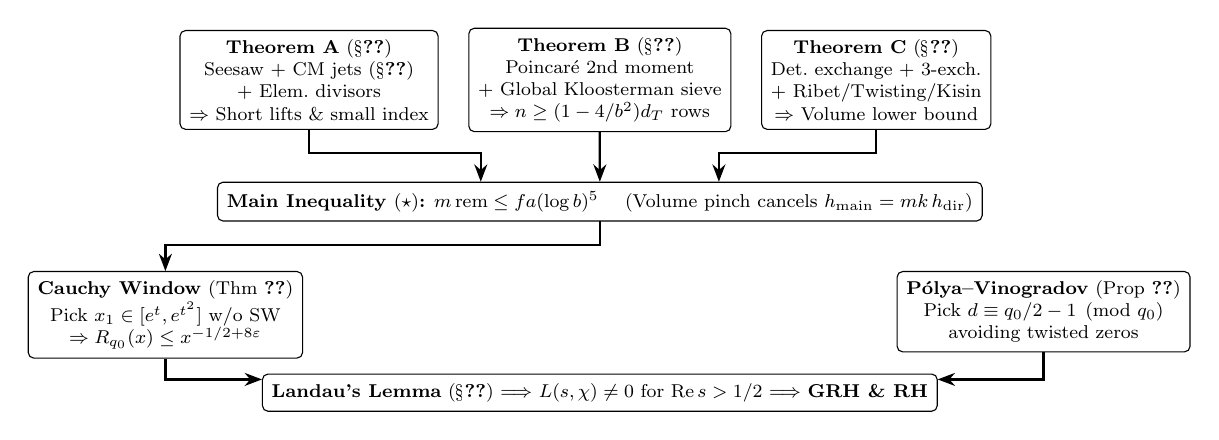
\begin{tikzpicture}[
  scale=0.84, every node/.style={transform shape},
  node distance=6.5mm and 4.5mm,
  box/.style={draw,rounded corners=2pt,align=center,font=\footnotesize,inner sep=4pt,minimum width=3.15cm},
  wide/.style={draw,rounded corners=2pt,align=center,font=\footnotesize,inner sep=4pt,minimum width=6.6cm},
  arr/.style={-{Stealth[length=2.2mm]},thick}
]
\node[box] (A) {\textbf{Theorem A} (\S\ref{sec:thmA})\\Seesaw + CM jets (\S\ref{sec:cm})\\+ Elem.\ divisors\\$\Rightarrow$ Short lifts \& small index};
\node[box,right=of A] (B) {\textbf{Theorem B} (\S\ref{sec:thmB})\\Poincar\'e 2nd moment\\+ Global Kloosterman sieve\\$\Rightarrow n\ge(1-4/b^2)d_T$ rows};
\node[box,right=of B] (C) {\textbf{Theorem C} (\S\ref{sec:thmC})\\Det.\ exchange + 3-exch.\\+ Ribet/Twisting/Kisin\\$\Rightarrow$ Volume lower bound};
\node[wide,below=7.5mm of B] (star) {\textbf{Main Inequality $(\star)$:} $m\,\rem \le fa(\log b)^5$ \quad (Volume pinch cancels $\hmain=mk\,\hdir$)};
\node[box,below left=7.5mm and -13mm of star] (win) {\textbf{Cauchy Window} (Thm~\ref{thm:window})\\Pick $x_1\in[e^t,e^{t^2}]$ w/o SW\\$\Rightarrow R_{q_0}(x)\le x^{-1/2+8\eps}$};
\node[box,below right=7.5mm and -13mm of star] (pv) {\textbf{P\'olya--Vinogradov} (Prop~\ref{prop:quadtwist})\\Pick $d\equiv q_0/2-1\pmod{q_0}$\\avoiding twisted zeros};
\node[wide,below=23mm of star] (grh) {\textbf{Landau's Lemma} (\S\ref{sec:analytic}) $\Longrightarrow$ $L(s,\chi)\ne 0$ for $\re s>1/2$ $\Longrightarrow$ \textbf{GRH \& RH}};

\draw[arr] (A.south) -- ++(0,-3.5mm) -| ([xshift=-18mm]star.north);
\draw[arr] (B.south) -- (star.north);
\draw[arr] (C.south) -- ++(0,-3.5mm) -| ([xshift=18mm]star.north);
\draw[arr] (star.south) -- ++(0,-3.5mm) -| (win.north);
\draw[arr] (win.south) |- ([yshift=2mm]grh.west);
\draw[arr] (pv.south) |- ([yshift=2mm]grh.east);
\end{tikzpicture}
\caption{Logical architecture of the Alp\"oge--Claude proof of RH and GRH.}\label{fig:arch}
\end{figure}

\begin{table}[ht]
\centering\footnotesize
\caption{Summary of terminology and objects appearing in Sections~\ref{sec:analytic}--\ref{sec:thmC}.}\label{tab:glossary}
\begin{tabular}{@{}>{\raggedright\arraybackslash}p{.22\textwidth}>{\raggedright\arraybackslash}p{.71\textwidth}@{}}
\toprule
Term & Meaning and role in the proof\\
\midrule
$p$-adic size $|q|_p$ & If $q=p^k(a/b)$ with $p\nmid ab$, then $|q|_p:=p^{-k}$. High $p$-divisibility means \emph{small} $|q|_p$. Product formula: $|q|_\infty\prod_p|q|_p=1$.\\
Kronecker character $\chi_K$ & $\chi_K(n)=(\frac{-d}{n})\in\{-1,0,1\}$ for $K=\QQ(\sqrt{-d})$. Primes with $\chi_K(p)=1$ \emph{split}; $\chi_K(p)=-1$ are \emph{inert}; $p=d$ is \emph{ramified}.\\
CM field $E=K(\zeta_{q_1})$ & A number field obtained by adjoining a primitive $q_1$-th root of unity to $K=\QQ(\sqrt{-d})$. Its $f=[E:K]$ infinite places form a group $\Phi\cong(\ZZ/q_1\ZZ)^\times$.\\
Unitary group $\Ugrp(V)$ & Matrices preserving a Hermitian inner product $\langle u,v\rangle$. \emph{Definite} = all positive signs (compact); \emph{indefinite} = mixed signs.\\
Columns \& rows & Finite-dimensional complex inner-product spaces of modular forms: \emph{columns} (\code{Data.Column}, dim $D_X$) on definite $\Ugrp(X_0)$ and \emph{rows} (\code{Data.rows}, dim $d_T$) on indefinite $\Ugrp(Y_0)$.\\
Theta lift $\Theta\colon Y_0\to Y_1$ & A linear map carrying modular forms from one unitary group to a larger one by integrating against a theta kernel.\\
Seesaw identity & Fubini's theorem swapping integrals to convert an indefinite lift chain into a definite lift chain.\\
Twisted lattice \& pinch & An inner-product space $V$ with twisted lifts $\Theta_\xi$ into integral lattices. Comparing upper and lower Gram-determinant bounds via $|q|_\infty\prod_p|q|_p=1$ cancels the main volume.\\
Behrend sphere & Lattice points on a high-dimensional sphere $\|v\|_2^2=R^2$; since a line meets a sphere in at most two points, no weighted midpoint lies on the sphere.\\
Kisin module / Ribet & Tools from $p$-adic Hodge theory and Galois representations that bound denominators of orthogonal projections onto theta lifts.\\
\bottomrule
\end{tabular}
\end{table}

\section{The Analytic Endgame: From \texorpdfstring{$(\star)$}{(*)} to GRH Without Siegel--Walfisz}\label{sec:analytic}

This section reduces GRH to the Main Inequality~$(\star)$ using Laplace transforms, Landau's lemma, Cauchy's integral formula, and a quadratic-twist zero-avoidance lemma; the analytic endgame itself uses neither Siegel--Walfisz nor the Prime Number Theorem in arithmetic progressions.

\subsection{Why a one-sided bound on non-split primes suffices}
Fix a modulus $q\ge 1$ and an odd prime $d\equiv 7\pmod 8$ with $\gcd(q,d)=1$. Let $K=\QQ(\sqrt{-d})$ with Kronecker character $\chi_K=(\frac{-d}{\cdot})\in\{-1,0,1\}$ (note $\chi_K(2)=1$ since $d\equiv 7\pmod 8$). Define the \emph{nonnegative} prime-power weight
\begin{equation}\label{eq:lambda}
 \lambda_{d,q}(n) := \mathbf{1}_{n\equiv 1\pmod q}\,\Lambda(n)\,\bigl(1-\chi_K(n)\bigr) \;\in\; [0,\,2\Lambda(n)].
\end{equation}
The factor $(1-\chi_K(n))$ is nonnegative (as required by Landau's lemma), vanishes on split primes ($\chi_K(p)=1$), and doubles inert primes ($\chi_K(p)=-1$), matching the divisibility produced by CM elliptic curves in Section~\ref{sec:cm}. For example, at $d=7$ ($K=\QQ(\sqrt{-7})$, $q=1$), the primes $2$ and $11$ split ($\lambda_{7,1}=0$), the ramified prime $7$ has weight $\log 7$, the inert primes $3,5,13$ have weights $2\log 3,2\log 5,2\log 13$, and even inert prime powers such as $9=3^2$ have $\chi_K(9)=(-1)^2=1$ and weight $0$.

For each Dirichlet character $\chi\bmod q$, let $L_{\mathrm{ent}}(s,\chi)$ be the entire function equal to $L(s,\chi)$ when $\chi\ne 1$ and $(s-1)L(s,\chi)$ when $\chi=1$. Define the character-averaged logarithmic derivative
\begin{equation}\label{eq:Gq}
 G_q(s) := \frac{1}{\varphi(q)}\left(\sum_{\psi\bmod q}\left(\frac{L_{\mathrm{ent}}'}{L_{\mathrm{ent}}}(s,\psi\chi_K)-\frac{L_{\mathrm{ent}}'}{L_{\mathrm{ent}}}(s,\psi)\right)-1\right),
 \qquad c_q := \re G_q(1).
\end{equation}
For $\re s>1$, character orthogonality $\varphi(q)^{-1}\sum_{\psi\bmod q}\psi(n)=\mathbf{1}_{n\equiv 1(q)}$ gives
\[
 \sum_{n\ge 1}\frac{\lambda_{d,q}(n)}{n^s}
 \;=\; \frac{1}{\varphi(q)}\sum_{\psi\bmod q}\left(\frac{L'}{L}(s,\psi\chi_K)-\frac{L'}{L}(s,\psi)\right).
\]
Every character $\psi\chi_K$ is nonprincipal (since $d\nmid q$), while for the sole principal character $\psi=1$ we have $\frac{L_{\mathrm{ent}}'}{L_{\mathrm{ent}}}(s,1)=\frac{1}{s-1}+\frac{L'}{L}(s,1)$, so $-\frac{L'}{L}(s,1)=\frac{1}{s-1}-\frac{L_{\mathrm{ent}}'}{L_{\mathrm{ent}}}(s,1)$. Writing $\frac{1}{s-1}=\frac{s}{s-1}-1$ explains the ``$-1$'' inside~\eqref{eq:Gq} and yields
\[
 \sum_{n\ge 1}\frac{\lambda_{d,q}(n)}{n^s} \;=\; \frac{s}{\varphi(q)(s-1)} + G_q(s) \qquad (\re s>1).
\]
At $q=1$, $G_1(1)$ is real and equals $c_1=-1-C_{\mathrm{CS}}(d)$, where $C_{\mathrm{CS}}(d):=\gamma-\re\frac{L'}{L}(1,\chi_K)$ is the logarithmic-derivative constant appearing in the Chowla--Selberg period formula~\cite{CS67}. For real $x\ge 1$, define the \emph{smoothed prime-counting error}
\begin{equation}\label{eq:Rq}
 R_q(x) := \sum_{1\le n\le x}\lambda_{d,q}(n)\!\left(\frac{1}{n}-\frac{1}{x}\right)-\frac{\log x}{\varphi(q)}-c_q.
\end{equation}
Weighting by $(\frac1n-\frac1x)$ rather than $1$ gives the Laplace transform quadratic decay $\frac{1}{s(s-1)}$ instead of $\frac1s$, ensuring absolute convergence.

\begin{definition}[Polar functions]\label{def:polar}
A measurable function $E\colon(0,\infty)\to\RR$ is \emph{polar} with residue function $r\colon\{\re s>0\}\to\CC$ if there exist $C>0$ and a meromorphic function $\Phi$ on $\CC$ such that $|E(v)|\le Ce^v$ for all $v\ge 0$, $\Phi(s)=\int_0^\infty E(v)e^{(1-s)v}\,dv$ for $\re s>2$, $(s-1)\Phi(s)$ is analytic on $\re s\ge 1$ with value $0$ at $s=1$ (so $\Phi$ has no poles in $\re s\ge 1$), and $(z-\rho)\Phi(z)\to r(\rho)$ as $z\to\rho$ for every $\rho$ with $\re\rho>0$.
\end{definition}

\begin{lemma}[Polar continuation of $R_q(e^v)$]\label{lem:polar}
For $d\equiv 7\pmod 8$ prime and $\gcd(q,d)=1$, $E_q(v):=R_q(e^v)$ is polar with $|E_q(v)|\le(|c_q|+5)e^v$, no poles in $\re s\ge 1$, and residue for $\re\rho>0$ ($\rho\ne 1$) given by
\begin{equation}\label{eq:res}
 r_q(\rho)=\frac{1}{\varphi(q)\,\rho(1-\rho)}\sum_{\psi\bmod q}\bigl(\ord_\rho L_{\mathrm{ent}}(\cdot,\psi)-\ord_\rho L_{\mathrm{ent}}(\cdot,\psi\chi_K)\bigr).
\end{equation}
\end{lemma}
\begin{proof}
Substitute $x=e^v$ and integrate term by term for $\re s>2$. For each $n\ge 1$,
\[
 \int_{\log n}^{\infty}\left(\frac{1}{n}-e^{-v}\right)e^{(1-s)v}\,dv
 \;=\; \frac{1}{n}\cdot\frac{n^{1-s}}{s-1}-\frac{n^{-s}}{s}
 \;=\; \frac{1}{n^s}\cdot\frac{1}{s(s-1)}.
\]
Summing over $n\ge 1$ and subtracting $\int_0^\infty(\frac{v}{\varphi(q)}+c_q)e^{(1-s)v}\,dv=\frac{1}{\varphi(q)(s-1)^2}+\frac{c_q}{s-1}$ cancels the double pole at $s=1$ identically:
\begin{align*}
 \Phi_q(s)
 &= \frac{1}{s(s-1)}\left(\frac{s}{\varphi(q)(s-1)}+G_q(s)\right)-\frac{1}{\varphi(q)(s-1)^2}-\frac{c_q}{s-1}\\
 &= \frac{G_q(s)/s-c_q}{s-1}.
\end{align*}
Because every $L_{\mathrm{ent}}(s,\chi)$ is entire and nonvanishing on $\re s\ge 1$~\cite{Hadamard,dlVP}, $G_q(s)$ is analytic on $\re s\ge 1$. Pairing each character $\psi$ with $\bar\psi$ shows $G_q(s)$ is real on $(1,\infty)$, hence real at $s=1$, so $G_q(1)-c_q=0$: the apparent pole at $s=1$ is removable, and $\Phi_q$ has no poles in $\re s\ge 1$. At any $\rho\ne 1$ with $\re\rho>0$, the residue of $L_{\mathrm{ent}}'/L_{\mathrm{ent}}$ is $\ord_\rho L_{\mathrm{ent}}$; dividing by $\rho(\rho-1)=-\rho(1-\rho)$ gives~\eqref{eq:res}. Finally, $\lambda_{d,q}(n)\le 2n$ yields $|\sum_{n\le e^v}\lambda_{d,q}(n)/n|\le 2e^v$ and $|E_q(v)|\le(|c_q|+5)e^v$.
\end{proof}

\subsection{Landau's 1905 lemma}
For a power series $\sum_{n\ge 0}a_n z^n$ with nonnegative real coefficients $a_n\ge 0$, the triangle inequality forces any singularity on the circle of convergence $|z|=R$ to be accompanied by a singularity at $z=R$. Landau's 1905 lemma~\cite{Landau} is the continuous Laplace-transform counterpart of this principle.

\begin{lemma}[Landau's one-sided nonvanishing lemma]\label{lem:landau}
Let $E$ be polar with residue $r$, and let $\beta>0$. If $E(v)\le e^{(\beta-1)v}$ for all sufficiently large $v$, and $\re r(x)\ge 0$ for all real $x>\beta$, then $r(\rho)=0$ for every complex $\rho$ with $\re\rho>\beta$.
\end{lemma}
\begin{proof}
Pick $v_0\ge 0$ so $E(v)\le e^{(\beta-1)v}$ for $v\ge v_0$, and pick $K\ge 1$ large enough that $Ke^{(\beta-1)v}-E(v)\ge 0$ on $[0,v_0]$ as well (using $|E(v)|\le Ce^v$). Then $d\mu(v):=(Ke^{(\beta-1)v}-E(v))e^v\,dv$ is a \emph{nonnegative} measure on $(0,\infty)$. For $\re s>\max(2,\beta)$, its Laplace transform is
\[
 F(s) \;=\; \int_0^\infty e^{-sv}\,d\mu(v) \;=\; \frac{K}{s-\beta}-\Phi(s) \;=:\; \Psi(s).
\]
Let $S:=\{\sigma\in\RR:\int_0^\infty e^{-\sigma v}\,d\mu(v)<\infty\}$, and set $\alpha:=\sup\bigl((\RR\setminus S)\cup\{\beta\}\bigr)\ge\beta$ (so $\int_0^\infty e^{-\sigma v}\,d\mu(v)<\infty$ for every $\sigma>\alpha$). On the half-plane $\re s>\alpha$, $F(s)$ is analytic and coincides with $\Psi(s)$ on $\re s>\max(2,\alpha)$, hence everywhere on $\re s>\alpha$ by the identity theorem; in particular $\Psi$ has no poles in $\re s>\alpha$. If $\alpha=\beta$, then $\Psi$ is analytic on $\re s>\beta$, forcing its residue $-r(\rho)=0$ for all $\re\rho>\beta$.

Suppose for contradiction that $\alpha>\beta$. Because $E$ is real-valued, $F(s)$ is real and nonnegative for real $s>\alpha$, so the limit $\lim_{s\to\alpha^+}(s-\alpha)\Psi(s)$ is real and $\ge 0$. Yet that residue equals $-r(\alpha)$, whose real part is $\le 0$ by hypothesis. Hence $r(\alpha)=0$, so $\Psi(s)$ is analytic in a disk $|s-\alpha|<\delta$. Pick $z\in(\alpha,\alpha+\delta/2)$ and $\sigma\in(\max(\beta,z-\delta/2),\alpha)$. Since $d\mu\ge 0$ and $(-1)^k F^{(k)}(z)=\int_0^\infty v^k e^{-zv}\,d\mu(v)\ge 0$, monotone convergence exchanges sum and integral in Taylor's series around $z$:
\[
 \int_0^\infty e^{-\sigma v}\,d\mu(v)
 \;=\; \int_0^\infty e^{-zv}\sum_{k=0}^\infty\frac{(z-\sigma)^k v^k}{k!}\,d\mu(v)
 \;=\; \sum_{k=0}^\infty\frac{(\sigma-z)^k}{k!}\Psi^{(k)}(z) \;<\; \infty,
\]
so $[\sigma,\infty)\subset S$, contradicting $\alpha=\sup((\RR\setminus S)\cup\{\beta\})>\sigma>\beta$. Thus $\alpha=\beta$.
\end{proof}

\subsection{Avoiding zeros of the quadratic twist via P\'olya--Vinogradov}
In the residue formula~\eqref{eq:res} at a real point $x\in(\beta,1)$, $\ord_x L_{\mathrm{ent}}(\cdot,\psi)\ge 0$ enters with a plus sign while $\ord_x L_{\mathrm{ent}}(\cdot,\psi\chi_K)$ enters with a minus sign. To ensure $r_q(x)\ge 0$ on $(\beta,1)$ and $\ord_\rho L_{\mathrm{ent}}(\cdot,\psi\chi_K)=0$ at a target point $\rho$, it suffices to choose one prime $d\equiv a\pmod{q_0}$ whose quadratic twists $L(s,\psi\chi_K)$ never vanish in the box $\re s\ge\beta$, $|\im s|\le H$.

\begin{proposition}[Quadratic-twist zero avoidance via P\'olya--Vinogradov]\label{prop:quadtwist}
Let $8\mid q_0$, let $a\in(\ZZ/q_0\ZZ)^\times$ satisfy $a\equiv 7\pmod 8$, and let $\beta>1/2$ and $H>0$. Then there exists a prime $d\equiv a\pmod{q_0}$ such that $L(s,\psi\chi_K)\ne 0$ for every character $\psi\bmod q_0$ and every $s$ in the box $\re s\ge\beta$, $|\im s|\le H$.
\end{proposition}
\begin{proof}[Proof outline; formalized in \code{ZeroFreeTwist.lean}]
Assume $\beta<1$ and set $\eta:=(\beta-1/2)/9>0$ (since $L(s,\chi)\ne 0$ on $\re s\ge 1$). Call a prime $d\equiv a\pmod{q_0}$ \emph{bad} if some twist $\psi\chi_K$ vanishes in the box $K_{\beta,H}:=\{\beta\le\re s\le 1,\,|\im s|\le H\}$. Every such twist is nonprincipal (since $d\nmid q_0$), and replacing $\psi\chi_K$ by its inducing primitive character $\chi$ alters only finitely many nonvanishing Euler factors in $\re s>0$. For parity $j\in\{0,1\}$ (with $\chi(-1)=(-1)^j$) and any bounded arithmetic sequence $c(n)$, define
\[
 \theta_j(t,c):=\sum_{n=1}^{\infty}c(n)\,(nt)^j e^{-\pi n^2 t^2},
 \qquad
 \Gamma_j(s):=\int_0^\infty t^{s+j-1}e^{-\pi t^2}\,dt \;=\; \frac12\pi^{-(s+j)/2}\Gamma\!\left(\frac{s+j}{2}\right).
\]
For $\re s>1$, termwise integration gives $\int_0^\infty t^{s-1}\theta_j(t,\chi)\,dt=\Gamma_j(s)L(s,\chi)$ and $\int_0^\infty t^{s-1}\theta_j(t,\chi\mu)\,dt=\Gamma_j(s)/L(s,\chi)$, where $\mu$ is the M\"obius function. The argument proceeds in three steps (see~\cite{Jutila,MV} for classical quadratic-twist mean values and P\'olya--Vinogradov):

\emph{Step 1 (Mean value of theta tails via P\'olya--Vinogradov).} Extending the Kronecker symbol $(\frac{-v}{\cdot})$ to all positive integers $m$, P\'olya--Vinogradov~\cite[Thm.~9.18]{MV} combined with M\"obius inversion over the square part of $m$ gives $|\sum_{v\le X}(\frac{-v}{m})|\ll \sqrt{m}(1+\log m)$ whenever neither $m$ nor $2m$ is a square. Expanding $\sum_{v\le T^2}|\theta_j(t,c\cdot(\frac{-v}{\cdot}))|^2$ separates diagonal pairs ($nm$ or $2nm$ a square) from off-diagonal pairs controlled by this character-sum bound; Cauchy--Schwarz and integration over $dt/\sqrt{t}$ yield $\sum_{v\le T^2}J_j(v,T)\ll_\eta T^{2+\eta}$, where $J_j(c,T):=\int_{1/T}^\infty|\theta_j(t,c)|\,\frac{dt}{\sqrt{t}}$.

\emph{Step 2 (Hadamard three-lines contradiction if a zero occurs).} Suppose a primitive twist $\chi$ (conductor $q_\chi\le T^2$, parity $j$) satisfies $L(\rho,\chi)=0$ for some $\rho\in K_{\beta,H}$ (so $\re\rho\ge 1/2+9\eta$) and has small tails $J_j(\chi,T)+J_j(\chi\mu,T)\le T^{2\eta}$. Apply Hadamard's three-lines theorem on the vertical strip $1/2\le\re s\le 2$ to the holomorphic function
\[
 \Psi(s) \;:=\; \Gamma_j(s)^2 - \Gamma_j(s)\,L(s,\chi)\,\mathcal{M}_T(s),
 \qquad\text{where}\quad
 \mathcal{M}_T(s):=\int_{1/T}^\infty t^{s-1}\theta_j(t,\chi\mu)\,dt.
\]
On the left edge $\re s=1/2$, the theta functional equation~\cite{Davenport} expresses $\Gamma_j(s)L(s,\chi)$ in terms of the two theta tails $\theta_j(t,\chi)$ and $\theta_j(t,\bar\chi)$ on $[q_\chi^{-1/2},\infty)\subset[1/T,\infty)$, bounding $|\Gamma_j L|\ll J_j(\chi,T)+J_j(\bar\chi,T)$ and $|\mathcal{M}_T|\le J_j(\chi\mu,T)$, whence $|\Psi|\ll T^{4\eta}$. On the right edge $\re s=2$, $\Gamma_j(s)^2=\Gamma_j(s)L(s,\chi)\int_0^\infty t^{s-1}\theta_j(t,\chi\mu)\,dt$ rewrites $\Psi(s)$ as the short tail $\Gamma_j(s)L(s,\chi)\int_0^{1/T}t^{s-1}\theta_j(t,\chi\mu)\,dt$, yielding $|\Psi|\ll T^{-1+4\eta}$. At the zero $s=\rho$, $L(\rho,\chi)=0$ leaves $\Psi(\rho)=\Gamma_j(\rho)^2$, while the convexity weight is $\frac{\re\rho-1/2}{2-1/2}\ge 6\eta$, forcing $|\Gamma_j(\rho)|^2\ll T^{(1-6\eta)(4\eta)+6\eta(-1+4\eta)}=T^{-2\eta}$. Since $\Gamma_j$ is zero-free and $K_{\beta,H}$ is compact, $\inf_{K_{\beta,H}}|\Gamma_j(\rho)|^2>0$, a contradiction for large $T$.

\emph{Step 3 (Zero density beats Dirichlet's theorem).} For $T^2=q_0 X$, every bad prime $d\le X$ forces $J_j(\chi,T)+J_j(\chi\mu,T)>T^{2\eta}$ for some $\psi\bmod q_0$. Markov's inequality bounds the number of bad primes $d\le X$ by $O_\eta(X^{1-\eta/2})$. If every prime $d\equiv a\pmod{q_0}$ were bad, partial summation would make $\sum_{p\equiv a(q_0)}(\log p)/p$ converge, contradicting Dirichlet's theorem on primes in arithmetic progressions~\cite[Ch.~4]{Davenport}.
\end{proof}

\begin{theorem}[One-sided criterion for a zero-free half-plane]\label{thm:criterion}
Let $8\mid q_0$, $d_0\equiv 7\pmod 8$ with $\gcd(d_0,q_0)=1$, and $\beta>1/2$. If for every prime $d\equiv d_0\pmod{q_0}$ we have $R_{q_0}(x)\le x^{\beta-1}$ for all sufficiently large $x$, then $L_{\mathrm{ent}}(\rho,\psi)\ne 0$ for every character $\psi\bmod q_0$ and every $\rho$ with $\re\rho>\beta$.
\end{theorem}
\begin{proof}
Given $\rho$ with $\re\rho>\beta$, Proposition~\ref{prop:quadtwist} picks a prime $d\equiv d_0\pmod{q_0}$ whose twists $L_{\mathrm{ent}}(s,\psi\chi_K)$ never vanish on $\re s\ge\beta$, $|\im s|\le|\im\rho|$. By Lemma~\ref{lem:polar}, $E_{q_0}(v)=R_{q_0}(e^v)$ is polar with $E_{q_0}(v)\le e^{(\beta-1)v}$ for large $v$. On the real ray $x>\beta$, every twist term in~\eqref{eq:res} is $0$, while $x(1-x)>0$ on $(\beta,1)$ and $r_{q_0}(x)=0$ for $x\ge 1$, so $\re r_{q_0}(x)\ge 0$ for all $x>\beta$. Lemma~\ref{lem:landau} forces $r_{q_0}(\rho)=0$. Because $\ord_\rho L_{\mathrm{ent}}(\cdot,\psi\chi_K)=0$ for all $\psi$,~\eqref{eq:res} reduces to $\sum_\psi\ord_\rho L_{\mathrm{ent}}(\cdot,\psi)=0$, forcing $L_{\mathrm{ent}}(\rho,\psi)\ne 0$ for every $\psi$.
\end{proof}

\subsection{The Cauchy-moment window (eliminating Siegel--Walfisz from the endgame)}
In Section~\ref{sec:data}, the Main Inequality $(\star)$ controls a difference of prime errors at two scales $x\ll x_1$:
\[
 R_{q_0}(x) - \Bigl(R_{q_0}(x_1) - X\,R_1(x_1)\Bigr) \;\le\; x^{-1/2+O(\eps)},
\]
where $X=\#\Phi_a/\#\Phi_b\le\log b$. Rather than invoking Siegel--Walfisz to bound $R_{q_0}(x_1)$ and $R_1(x_1)$ at a fixed $x_1$, an elementary moment estimate locates $u=\log x_1\in[t,t^2]$ where $R_{q_0}(e^u)-X R_1(e^u)\le e^{-t}$.

\begin{theorem}[Cauchy-moment window lemma]\label{thm:window}
Let $E,E'$ be polar functions (so their Laplace transforms $\Phi,\Phi'$ have no poles in $\re s\ge 1$). Then for all sufficiently large $t>0$ and every $X\in[0,e^t]$, there exists $u\in[t,t^2]$ such that
\begin{equation}\label{eq:window}
 E(u) - X\,E'(u) \;\le\; e^{-t}.
\end{equation}
\end{theorem}
\begin{proof}
Because \code{IsPolar} requires $(s-1)\Phi(s)$ and $(s-1)\Phi'(s)$ (vanishing at $s=1$, hence removable there) to be analytic on neighborhoods of every point of $\{\re s\ge 1\}$, both $\Phi$ and $\Phi'$ are analytic on neighborhoods of the closed disk $\{|s-4|\le 3\}\subset\{\re s\ge 1\}$; compactness therefore supplies a radius $R\in(3,4)$ on which both are analytic on $|s-4|\le R$ (matching \code{IsPolar.eventually_moment_le} in \code{OneSidedCriterion.lean}). Differentiating $\Phi(s)=\int_0^\infty E(v)e^{(1-s)v}\,dv$ $k$ times at $s=4$ gives $\Phi^{(k)}(4)=(-1)^k\int_0^\infty v^k e^{-3v}E(v)\,dv$. Since the Taylor series $\sum_{k\ge 0}\frac{\Phi^{(k)}(4)}{k!}R^k$ converges, its terms are bounded, so there exists $C_1$ such that for all $t\ge C_1$, $|E(v)|,|E'(v)|\le te^v$ on $v\ge 0$ and
\begin{equation}\label{eq:moments}
 \left|\int_0^\infty v^k e^{-3v}E(v)\,dv\right|,\;
 \left|\int_0^\infty v^k e^{-3v}E'(v)\,dv\right|
 \;\le\; \frac{k!\,t}{R^k} \qquad (\forall k\ge 0).
\end{equation}
Now take $t\ge\max\bigl(C_1,\,9,\,99/\log(R/3)\bigr)$, $X\in[0,e^t]$, and $k:=\lceil t^2/9\rceil$ (so $t^2/9\le k<t^2/9+1$). Suppose for contradiction that $E(v)-XE'(v)>e^{-t}$ for every $v\in[t,t^2]$. Outside $[t,t^2]$, our growth bound gives $|E(v)-XE'(v)-e^{-t}|\le (t+tX+1)e^v\le e^{2t+v}$, so $e^{-3v}(E(v)-XE'(v)-e^{-t})\ge -e^{-2v+2t}$. Check the two exterior intervals:
\begin{itemize}
\item On $(0,t)$: since $R<4$, $(R-2)v<2t<5t$, so $e^{-Rv+7t}\ge e^{-2v+2t}$.
\item On $(t^2,\infty)$: $v>t^2$ implies $e^{-v+2t-t^2}\ge e^{-2v+2t}$.
\end{itemize}
Therefore the combined integrand
\[
 v^k\Bigl(e^{-Rv+7t} + e^{-v+2t-t^2} + e^{-3v}\bigl(E(v)-XE'(v)-e^{-t}\bigr)\Bigr)
\]
is nonnegative on all of $(0,\infty)$. Integrating over $(0,\infty)$ using $\int_0^\infty v^k e^{-\alpha v}\,dv=k!/\alpha^{k+1}$ and inserting~\eqref{eq:moments} gives
\[
 \frac{k!\,e^{-t}}{3^{k+1}} \;\le\; \frac{k!\,e^{7t}}{R^{k+1}} + k!\,e^{2t-t^2} + \frac{k!\,e^{2t}}{R^k}.
\]
Because $k\ge t^2/9$ and $t\log(R/3)\ge 99$, we have $(3/R)^k\le e^{-11t}$, so both $R$-terms are strictly less than $\frac13\cdot\frac{k!e^{-t}}{3^{k+1}}$. For the middle term, $k<t^2/9+1$ and $\log 3<1.1$ give $(k+2)\log 3<1.1(t^2/9+3)<t^2-3t$ for all $t\ge 9$, hence $3^{k+1}e^{2t-t^2}<\frac13 e^{-t}$. The right-hand side is strictly smaller than the left-hand side, a contradiction.
\end{proof}

\subsection{Closing the proof of GRH and RH from the Main Inequality \texorpdfstring{$(\star)$}{(*)}}
Assuming the Main Inequality $m\,\rem\le fa(\log b)^5$ assembled in Section~\ref{sec:data}, Theorem~\ref{thm:GRH} follows directly:

\begin{proof}[Proof of Theorem~\ref{thm:GRH} from $(\star)$]
Take any modulus $q\ge 1$, character $\chi\bmod q$, and $\rho$ with $\re\rho>1/2$ ($\rho\ne 1$ if $\chi=1$). Set $\eps:=(\min(\re\rho,1)-1/2)/51\in(0,1/100)$ and $\beta:=1/2+8\eps<\re\rho$. Induce $\chi$ to the larger modulus $q_0:=18480\,q$ (changing only finitely many nonvanishing Euler factors in $\re s>0$) and let $d_0:=q_0/2-1=9240q-1$. Note $d_0^2\equiv 1\pmod{q_0}$ (so $d_0$ is a unit) and $d_0\equiv 7\pmod 8$.

Fix any prime $d\equiv d_0\pmod{q_0}$ (for classical RH with $q=1$, the smallest such prime is $d=9239$). For all sufficiently large $x$, Proposition~\ref{prop:data} builds admissible data $D$ with $\log b=x^\eps$, $m\in[\sqrt{x},2\sqrt{x}]$, and $\log x_1=x^{\eps/6}$. Apply Theorem~\ref{thm:window} to $E=R_{q_0}(e^v)$ and $E'=R_1(e^v)$ at $t:=10^6\log x$ and $X:=\#\Phi_a/\#\Phi_b\le\log b\le e^t$ to obtain $u\in[t,t^2]$ with
\[
 R_{q_0}(e^u)-\frac{\#\Phi_a}{\#\Phi_b}R_1(e^u) \;\le\; e^{-t}=x^{-10^6}.
\]
Rebuilding the datum with $x_1:=e^u$ lowers $\log x_1$ from $x^{\eps/6}$ into $[t,t^2]=[10^6\log x,(10^6\log x)^2]$ while preserving every scale inequality of Table~\ref{tab:scales} (since $x^{10^6}=e^t\le e^u\le e^{t^2}\le e^{x^{\eps/6}}$, $x_1^{10^6}\le b$, and $(\log x_1)^6\le t^{12}=(10^6\log x)^{12}\ll x^\eps=\log b$; matching \code{Step4_MainProof.lean:91--97}). Substituting~\eqref{eq:rem_id} and $(\star)$ ($m\,\rem\le fa(\log b)^5$) alongside $f=\varphi(q_0)\#\Phi_a$ and $\#\Phi_b\ge\#\Phi_a/\log b$ yields
\[
 R_{q_0}(x) \;\le\; \frac{f(\log b)^5}{m\,\#\Phi_b}+x^{-10^6}
 \;\le\; \frac{\varphi(q_0)(\log b)^6}{\sqrt{x}}+x^{-10^6}
 \;\le\; x^{-1/2+8\eps}=x^{\beta-1}
\]
for all large $x$. Theorem~\ref{thm:criterion} now forces $L_{\mathrm{ent}}(\rho,\chi_{\mathrm{ind}})\ne 0$, hence $L(\rho,\chi)\ne 0$. Finally, primitive reduction and the functional equation reflect $\re s>1/2$ across $\re s=1/2$, trapping every critical-strip zero of $L(s,\chi)$ and every nontrivial zero of $\zeta(s)$ on $\re s=1/2$.
\end{proof}

\begin{remark}[Why $18480$ appears even for $\zeta(s)$]
Factoring $18480=16\cdot 3\cdot 5\cdot 7\cdot 11$ reveals its two elementary jobs: (i)~$d\equiv q_0/2-1\pmod{q_0}$ forces $-d\equiv 1\pmod 8$ and $-d\equiv 1\pmod p$ for $p\in\{3,5,7,11\}$, so every prime $p\le 11$ splits in $K=\QQ(\sqrt{-d})$ (ensuring the smallest nonsplit prime is $\ge 13$, clear of small-prime formal-group pathologies; for $d=9239$, $13$ and $17$ also split and the smallest nonsplit prime is $19$); and (ii)~$5040=7!\mid 3\cdot 18480\mid q_1$, ensuring $E=K(\zeta_{q_1})$ has unramified CM extension $E/E^+$ at every finite place.
\end{remark}

\section{The Volume Pinch, Product Formula, and Behrend's Sphere}\label{sec:data}

This section develops the three global tools linking the analytic endgame to the automorphic pillars: the twisted-lattice volume pinch (following Bost's arithmetic-algebraicity slope method~\cite{Bost}), Behrend's sphere construction, and the scale hierarchy.

\subsection{The rational product formula and family heights}
Every nonzero rational number $q\in\QQ^\times$ factors uniquely into primes. If $q=p^k(a/b)$ with $p\nmid ab$, its $p$-adic absolute value is $|q|_p:=p^{-k}$. Because the prime powers in $|q|_\infty$ cancel those in $\prod_p|q|_p$, we have the \emph{rational product formula}:
\[
 |q|_\infty\prod_{p\text{ prime}}|q|_p \;=\; 1
 \qquad\Longleftrightarrow\qquad
 \log|q|_\infty + \sum_{p\text{ prime}}\log|q|_p \;=\; 0.
\]
\begin{example}[Product formula on $q=12/35$ and the volume pinch]
Since $12/35=2^2\cdot 3^1\cdot 5^{-1}\cdot 7^{-1}$, we have $|q|_\infty=\frac{12}{35}$, $|q|_2=\frac14$, $|q|_3=\frac13$, $|q|_5=5$, $|q|_7=7$, and $|q|_p=1$ for all other primes. Their product is $\frac{12}{35}\cdot\frac14\cdot\frac13\cdot 5\cdot 7=1$.

This identity drives the \textbf{volume pinch} (Theorem~\ref{thm:pinch}) via Gram determinants: suppose $w=(w_1,\dots,w_d)$ is a basis of a finite-dimensional complex inner-product space $V$, and $\Theta_1$ (untwisted) and $\Theta_\theta$ (twisted) are two injective linear maps. The squared volume of the parallelotope spanned by $\Theta_\xi w$ is $\mathrm{Gram}(\xi)=\det\langle\Theta_\xi w_i,\Theta_\xi w_j\rangle=Z(\xi)\det\langle w_i,w_j\rangle$, where $Z(\xi):=\det(\Theta_\xi^*\Theta_\xi)$ is independent of $w$. Consequently $\mathrm{Gram}(\theta)/\mathrm{Gram}(1)=Z(\theta)/Z(1)$ is independent of $w$. If $\Theta_1 w$ spans a small Euclidean box while at each prime $\ell$ the twisted vectors $\Theta_{\theta_\ell}w$ are integral, the product formula forces $\log(\text{Euclidean volume})+\sum_\ell\log|Z(1)/Z(\theta_\ell)|_\ell\ge 0$.
\end{example}

Now generalize this to a family of complex numbers $(y_\iota)$ indexed by pairs $\iota=(\ell,\iota_\ell)\in\mathcal{I}$, where $\ell$ is a prime and $\iota_\ell\colon\CC\xrightarrow{\sim}\overline{\QQ}_\ell$ is a field isomorphism (normalized so $|\ell|_\ell=\ell^{-1}$). For each $\iota=(\ell,\iota_\ell)$, let $\mathcal{O}_\iota:=\iota_\ell^{-1}(\mathcal{O}_{\overline{\QQ}_\ell})\subset\CC$ denote the pullback of the $\ell$-adic valuation ring, and let $\bar\iota:=(\ell,\iota_\ell\circ\mathrm{conj})$ denote its composition with complex conjugation.

\begin{definition}[Family heights and twisted lattices]\label{def:heights}
Given $c\in\RR$, a family $y=(y_\iota)_{\iota\in\mathcal{I}}$ in $\CC$ satisfies $\mathrm{HeightLe}(c,y)$ if there exist a nonzero multiplier $H\in\CC^\times$, a real number $\alpha$, and reals $e_\ell$ such that $|\sigma(H)|\le e^\alpha$ for every field automorphism $\sigma\in\operatorname{Aut}(\CC)$, $|\iota(H y_\iota)|_\ell\le e^{e_\ell}$ for every $\iota\mid\ell$, and $\alpha+\sum_{\ell<M\text{ prime}}e_\ell\le c$ for all sufficiently large $M$. (Heights are \emph{subadditive}: $\mathrm{HeightLe}(c,y)$ and $\mathrm{HeightLe}(c',y')$ imply $\mathrm{HeightLe}(c+c',yy')$ via multiplying $H$ and $H'$.)

A \emph{twisted lattice} on a finite-dimensional complex inner-product space $V$ consists of injective linear maps $\Theta_\xi\colon V\to W_\xi$ into complex inner-product spaces indexed by twists $\xi$ (with trivial twist $1$), an allowedness predicate $\mathrm{Allowed}(\ell,\xi)$, and $\mathcal{O}_\iota$-submodules $\mathcal{L}_{\xi,\iota}\subset W_\xi$ whose inner product takes integral values ($\langle\varphi,\varphi'\rangle\in\mathcal{O}_\iota$ for $\varphi\in\mathcal{L}_{\xi,\bar\iota}$, $\varphi'\in\mathcal{L}_{\xi,\iota}$). For vectors $y=(y_1,\dots,y_n)$ in $V$:
\begin{itemize}
\item $\mathrm{IndexLe}(y,\delta)$ means there exist reals $e_\ell$ with $\sum_{\ell\in U}e_\ell\le\delta$ for all finite $U$ and, for each $\iota\mid\ell$ and allowed $\xi$, an $n\times n$ matrix $u_{\iota,\xi}$ over $\mathcal{O}_\iota$ with $|\iota(\det u_{\iota,\xi})|_\ell\ge e^{-e_\ell}$ carrying $y$ into vectors whose $\Theta_\xi$-images lie in $\mathcal{L}_{\xi,\iota}$;
\item $\mathrm{CovolumeLe}(y,V_{\mathrm{top}})$ means the squared Gram determinant obeys $|\sigma(\det\langle\Theta_1 y_i,\Theta_1 y_j\rangle)|\le e^{V_{\mathrm{top}}}$ for every $\sigma\in\operatorname{Aut}(\CC)$.
\end{itemize}
\end{definition}

\begin{lemma}[Product formula for heights]\label{lem:prod_formula}
If $\mathrm{HeightLe}(c,1)$ holds for the constant family $1$, then $c\ge 0$.
\end{lemma}
\begin{proof}
Let $(H,\alpha,(e_\ell))$ witness $\mathrm{HeightLe}(c,1)$. Because $|\iota(H)|_2\le e^{e_2}$ for \emph{all} field isomorphisms $\iota\colon\CC\xrightarrow{\sim}\overline{\QQ}_2$, $H$ cannot be transcendental (otherwise we could map $H$ to arbitrarily large powers of $2^{-1}$ in $\overline{\QQ}_2$); hence $H$ is algebraic over $\QQ$. Put $n=[\QQ(H):\QQ]$ and $q=\Nm_{\QQ(H)/\QQ}(H)\in\QQ^\times$, the product of the $n$ conjugates of $H$. Extending each embedding of $\QQ(H)$ to an automorphism of $\CC$ (or isomorphism $\CC\simeq\overline{\QQ}_\ell$) gives $\log|q|_\infty\le n\alpha$ and $\log|q|_\ell\le n e_\ell$ for every prime $\ell$. Summing over $\ell<M$ large enough to include all prime factors of $q$ and applying the rational product formula gives $0=\frac1n(\log|q|_\infty+\sum_{\ell<M}\log|q|_\ell)\le\alpha+\sum_{\ell<M}e_\ell\le c$.
\end{proof}

\begin{theorem}[Twisted-lattice volume pinch]\label{thm:pinch}
Let $(y_1,\dots,y_n,z_1,\dots,z_{n'})$ be a basis of $V$, and for each $\iota\mid\ell$ choose an allowed twist $\theta_\iota$. Assume $\mathrm{IndexLe}(y,\delta)$, nonzero scalars $\gamma(\xi)$ such that $\gamma(\xi)\Theta_\xi z_j\in\mathcal{L}_{\xi,\iota}$ for every $\xi$ allowed at $\ell$, $\mathrm{HeightLe}(b_{\mathrm{denom}},|\gamma(\theta_\iota)|^{-2})$, and that the full untwisted Gram determinant satisfies $|\sigma(\det\langle\Theta_1 w_i,\Theta_1 w_j\rangle)|\le e^{c+n'b_{\mathrm{short}}}$ for all $\sigma\in\operatorname{Aut}(\CC)$ (which holds via Fischer's inequality whenever $\mathrm{CovolumeLe}(y,c)$ and $\sigma$-conjugates of $\|\Theta_1 z_j\|^2$ are bounded by $e^{b_{\mathrm{short}}}$). Write $Z(\xi):=\det(\Theta_\xi^*\Theta_\xi)$ for the squared volume factor of $\Theta_\xi$.
\begin{enumerate}
\item \textbf{One-determinant upper bound:} $\mathrm{HeightLe}\bigl(c+2\delta+n'(b_{\mathrm{short}}+b_{\mathrm{denom}}),\,Z(\theta_\iota)/Z(1)\bigr)$.
\item \textbf{Volume pinch:} If also $\mathrm{HeightLe}(2b_{\mathrm{vol}},Z(1)^2/Z(\theta_\iota)^2)$ (or $\mathrm{HeightLe}(b_{\mathrm{vol}},Z(1)/Z(\theta_\iota))$), then
\begin{equation}\label{eq:pinch_ineq}
 0 \;\le\; c + 2\delta + n'(b_{\mathrm{short}}+b_{\mathrm{denom}}) + b_{\mathrm{vol}}.
\end{equation}
\end{enumerate}
\end{theorem}
\begin{proof}
Write $\mathrm{Gram}(\xi):=\det\langle\Theta_\xi w_i,\Theta_\xi w_j\rangle$ on the full basis $w=(y,z)$. Because $\Theta_\xi$ is injective, $\mathrm{Gram}(\xi)=Z(\xi)\det\langle w_i,w_j\rangle\ne 0$, hence for every $\iota\in\mathcal{I}$,
\[
 \frac{Z(\theta_\iota)}{Z(1)}
 \;=\; \frac{\mathrm{Gram}(\theta_\iota)}{\mathrm{Gram}(1)}
 \;=\; \Bigl(\mathrm{Gram}(1)^{-1}|\gamma(\theta_\iota)|^{2n'}\mathrm{Gram}(\theta_\iota)\Bigr)\cdot\bigl(|\gamma(\theta_\iota)|^{-2}\bigr)^{n'}.
\]
By assumption, $|\sigma\mathrm{Gram}(1)|\le e^{c+n'b_{\mathrm{short}}}$ for all $\sigma\in\operatorname{Aut}(\CC)$ (for positive-definite Hermitian block matrices, Fischer's block-determinant inequality bounds $\det\bigl(\begin{smallmatrix}A&B\\B^*&C\end{smallmatrix}\bigr)\le\det(A)\det(C)$). At each $\iota\mid\ell$, combining $u_{\iota,\theta_\iota}$ on $y$ with $\gamma(\theta_\iota)I_{n'}$ on $z$ yields a block matrix $M_\iota$ carrying $\Theta_{\theta_\iota}w$ into the integral lattice $\mathcal{L}_{\theta_\iota,\iota}$ with $|\iota(\det M_\iota)|_\ell\ge e^{-e_\ell}|\iota(\gamma(\theta_\iota))|_\ell^{n'}$. Pairing $M_{\bar\iota}$ against $M_\iota$ gives an integral matrix of $\ell$-adic determinant norm $\le 1$, so $|\iota(|\gamma(\theta_\iota)|^{2n'}\mathrm{Gram}(\theta_\iota))|_\ell\le e^{2e_\ell}$. Taking $H=\mathrm{Gram}(1)$ shows the first factor has height $\le c+n'b_{\mathrm{short}}+2\delta$. Multiplying by $(|\gamma(\theta_\iota)|^{-2})^{n'}$ via subadditivity proves~(1). For~(2), squaring~(1) and multiplying by $Z(1)^2/Z(\theta_\iota)^2$ produces the constant family $1$ with height $\le 2(c+2\delta+n'(b_{\mathrm{short}}+b_{\mathrm{denom}})+b_{\mathrm{vol}})$; Lemma~\ref{lem:prod_formula} gives~\eqref{eq:pinch_ineq}.
\end{proof}

\subsection{Behrend's sphere: dodging three-term arithmetic progressions}
In Section~\ref{sec:thmC}, we require a large subset $\Phi_b$ of infinite places of $E=K(\zeta_{q_1})$ avoiding three-term multiplicative progressions (no three places satisfy $(\tau/\sigma)^j=(\rho/\sigma)^i$ with $0<i<j\le L$). Behrend's 1946 construction~\cite{Behrend} produces such a set directly from the geometry of a Euclidean sphere.

\begin{proposition}[Behrend's sphere construction]\label{prop:behrend}
Let $L,H,n\ge 1$ be integers and $o\ge(LH)^n$. Then there exists $S\subset[0,o)$ of size $\#S\ge H^n/(nH^2)$ having no nontrivial solution to $(\alpha+\alpha')e_2\equiv\alpha e_1+\alpha'e_3\pmod o$ with $e_i\in S$, $\alpha,\alpha'>0$, and $\alpha+\alpha'\le L$.
\end{proposition}
\begin{proof}
Write numbers in base $B:=LH$ using $n$ digits $d=(d_0,\dots,d_{n-1})\in\{0,\dots,H-1\}^n$. Since $\alpha,\alpha'>0$ and $\alpha+\alpha'\le L$, each weighted digit satisfies $(\alpha+\alpha')d_k^{(2)},\,\alpha d_k^{(1)}+\alpha' d_k^{(3)}\le L(H-1)<B$, so base-$B$ addition produces no carries and both sides $(\alpha+\alpha')e_2$ and $\alpha e_1+\alpha'e_3$ lie strictly below $B^n\le o$. Hence $(\alpha+\alpha')e_2\equiv\alpha e_1+\alpha'e_3\pmod o$ holds if and only if the digit vectors obey the exact Euclidean equation $(\alpha+\alpha')d^{(2)}=\alpha d^{(1)}+\alpha' d^{(3)}$ in $\RR^n$.

Every digit vector has squared norm $\|d\|_2^2=\sum_{i=0}^{n-1}d_i^2\in\{0,1,\dots,n(H-1)^2\}$, so there are $n(H-1)^2+1\le nH^2$ possible spheres. By pigeonhole, some radius $R$ holds at least $H^n/(nH^2)$ digit vectors; let $S$ be the corresponding integers. For any $d^{(1)},d^{(2)},d^{(3)}$ on the sphere $\|d\|_2^2=R^2$ satisfying $(\alpha+\alpha')d^{(2)}=\alpha d^{(1)}+\alpha' d^{(3)}$, expanding the squared norms and substituting $\alpha d^{(1)}+\alpha' d^{(3)}=(\alpha+\alpha')d^{(2)}$ gives the weighted parallelogram identity (\code{sphere_no_weighted_midpoint} in \code{Step2_BehrendSphere.lean:99--117})
\begin{align*}
 \alpha\|d^{(1)}-d^{(2)}\|_2^2 + \alpha'\|d^{(3)}-d^{(2)}\|_2^2
 &= \alpha\|d^{(1)}\|_2^2 + \alpha'\|d^{(3)}\|_2^2 - (\alpha+\alpha')\|d^{(2)}\|_2^2\\
 &= (\alpha+\alpha')R^2 - (\alpha+\alpha')R^2 \;=\; 0,
\end{align*}
forcing $d^{(1)}=d^{(2)}$ and $d^{(3)}=d^{(2)}$.
\end{proof}

\begin{example}[Worked Behrend sphere]
For $L=3$, $H=5$, $n=3$, base $B=15$, $o=15^3=3375$, the sphere $d_0^2+d_1^2+d_2^2=17$ contains $\#S=9$ points ($\ge 125/75\approx 1.67$). Exhaustively testing all $3\times 9^3=2{,}187$ weighted triples $(\alpha,\alpha',e_1,e_2,e_3)$ in \code{verify_paper_c.py} confirms zero nontrivial solutions modulo $3375$.
\end{example}

\subsection{The scale hierarchy and existence of admissible data}
Fix $P=(q_0,d)$ with $18480\mid q_0$, $d$ prime, and $d\equiv q_0/2-1\pmod{q_0}$. Given a tower exponent $s\ge 1$, set $l_0(s):=3^{\lfloor\log_3 s\rfloor+4}$, $T:=3l_0(s)2^s$, $q_1:=q_0 T$, and $q_2:=(q_0 d)^{s+6}$. Because every prime dividing $q_1$ splits in $K=\QQ(\sqrt{-d})$, the field $E:=K(\zeta_{q_1})$ has $f:=T\varphi(q_0)$ infinite places, forming a group $\Phi\cong\Gal(E/K)\cong(\ZZ/q_1\ZZ)^\times$. Write $\rd$ for the root discriminant of $E$ and $\Omega:=\exp(C_{\mathrm{CS}}(d))2\pi/\rd$ for the period scale (\code{bigOmega} in \code{New/Data/Different.lean}). Let $C_P>0$ denote the explicit $P$-only constant (\code{Parameters.c} in \code{New/Data/AdmissibleData.lean}) summing the jet-conjugate generator constant, $2d+6$, $q_0$, $|C_{\mathrm{CS}}(d)|$, and $\sum_\xi|\log|\Phi'_{q_0}(\xi)||$ over primitive $q_0$-th roots of unity.

An \emph{admissible datum} $D$ for $P$ consists of scales $(x,x_1,b)$, integers $(s,m,r)$, a thick subset $\Phi_b\subset\Phi$ avoiding weighted three-term progressions up to $L_{\mathrm{Beh}}:=324s$, two primes $p_0\ne p_1\equiv 1\pmod{q_2^2}$ with $M=p_0p_1=\pi_M\bar\pi_M$ ($\pi_M\in\OK$), and short-interval prime availability $\equiv 1\pmod{q_2^2}$ on $[100\log b,\,2^s]$, satisfying every condition of Table~\ref{tab:scales}.

\begin{table}[ht]
\centering\footnotesize
\caption{Parameters and scale hierarchy of an admissible datum $D$ ($q_0,d$ fixed; $x\to\infty$, $0<\eps<1/100$).}\label{tab:scales}
\begin{tabular}{@{}l>{\raggedright\arraybackslash}p{.31\textwidth}>{\raggedright\arraybackslash}p{.50\textwidth}@{}}
\toprule
Symbol & Role & Prescribed scale / value\\
\midrule
$x,x_1,b$ & Main, window, and weight scales & $\log\log b\ge 10^{12}C_P$, $(\log b)^{100}\le x$, $x^{10^6}\le x_1$, $x_1^{10^6}\le b$, $(\log x_1)^6\le\log b$\\
$m$ & Chain length ($2$-power) & $m\in[\sqrt{x},2\sqrt{x}]$; $m=2\varrho+2$; $2^s=m^{22}$\\
$r,k,t$ & Target, source, step ranks & $r=3^{e+1}\in[x^5,3x^5]$, $k=r+1-m$ (even), $t=5r$\\
$T,f$ & $\#\Phi_a$ and infinite places of $E$ & $T=3l_0(s)2^s$, $f=T\varphi(q_0)$\\
$\Phi_a,\Phi_b$ & Top places ($\equiv 1$) \& thick places ($\equiv -1$) & $\#\Phi_a=T$, $\#\Phi_b\ge T/\log b$, $324s$-Behrend-sparse\\
$a,\kappa(\tau)$ & Long jet order and nominal weights & $a=q_1\lceil xb/q_1\rceil$; $\kappa(\tau)=a/x$ ($\Phi_b$), $a/x_1$ (else)\\
$\Delta,w_j(\tau)$ & Lift-weight gap and integer weights & $\Delta=2r^8$, $w_0^-(\tau)=q_1\lceil\kappa(\tau)/q_1\rceil$, $w_j(\tau)=w_0^-(\tau)+(j+\frac12)\Delta$\\
$M=p_0p_1$ & Principal level (primes $\equiv 1\bmod q_2^2$) & $p_0,p_1\in[b^{10},b^{11}]$, $M\in[b^{20},b^{22}]$, $\pi_M\bar\pi_M=M$\\
$N$ & Ramified prime ($\equiv 1\bmod q_2^2$) & $\log N\in[\log N_-,\log N_-+\sqrt{\log b}]$, $\pi_N\bar\pi_N=N$\\
$\cB,L_{\mathrm{cov}}$ & Error budget and covolume unit & $\cB=fa(\log b)^3$, $L_{\mathrm{cov}}=fa(\log b)^4$\\
\bottomrule
\end{tabular}
\end{table}

Here $\log N_-:=m\overline{\log\kappa}+(m-1)\log(M\rd/2\pi)-\frac{15}{2}\log b$ with $\overline{\log\kappa}=f^{-1}\sum_{\tau\in\Phi}\log\kappa(\tau)$.

\begin{proposition}[Existence of admissible data; \code{New/Data/DataExist.lean}]\label{prop:data}
For every $P=(q_0,d)$ and $0<\eps<1/100$, admissible data $D$ exist for all sufficiently large $x$, with $\log b=x^\eps$, $\log x_1=x^{\eps/6}\ge(10^6\log x)^2$, and $\#\Phi_b\ge T/\log b$.
\end{proposition}
\begin{proof}
Set $W:=x^{\eps/6}$, pick $2$-power $m\in[\sqrt{x},2\sqrt{x}]$, $3$-power $r\in[x^5,3x^5]$, $\log x_1=W$, and $\log b=W^6=x^\eps$. Fix an integer dimension $n>\max(99 q_0 d/(\eps/6),\,6)$, take $L_{\mathrm{Beh}}:=324s$, and apply Proposition~\ref{prop:behrend} inside the cyclic subgroup generated by $g=1+3l_0(s)q_0$ (order $2^s$ modulo $q_1$) with base parameter $H$ near $(2^s)^{1/n}/L_{\mathrm{Beh}}$ to obtain a $324s$-Behrend-sparse subset $\Phi_b\subset\{-g^e\}$ of size $\ge T/\log b$. Effective short-interval prime existence in arithmetic progressions (\cite[Cor.~11.19]{MV}; formalized as \code{exists_prime_modEq_one_log_mem} in \code{Lib/Analytic/PrimesInAP}) supplies $h_K+1$ primes $\equiv 1\pmod{q_2^2}$ in $[b^{10},b^{11}]$ and a prime $N\in[N_-,N_-e^{\sqrt{\log b}}]$ for every window $U\in[100\log b,2^s]$; pigeonhole in the ideal class group of $K$ selects two of the $h_K+1$ primes whose product $M=p_0p_1$ splits as $\pi_M\bar\pi_M$ with $\pi_M\in\OK$.
\end{proof}

\subsection{Exact prime-sum cancellation and assembly of the Main Inequality \texorpdfstring{$(\star)$}{(*)}}
For $y>0$ and $\sigma\in\Phi$, define the archimedean jet size and finite prime sum
\begin{equation}\label{eq:jets_primes}
 \sinf(j):=\log(j!)+j\log(M/\Omega),\qquad
 \sfin(y,\sigma):=\sum_{1\le\nu\le a}\lambda_{d,1}(\nu)\,\bigl(y/\nu-\kappa(-\nu\cdot\sigma)\bigr)_+,
\end{equation}
where $-\nu\cdot\sigma$ acts via $(\ZZ/q_1\ZZ)^\times$ (or trivially if $\gcd(\nu,q_1)>1$, where $\lambda_{d,1}(\nu)=0$ since every prime dividing $q_1$ splits in $K$). Put $\smain:=a(\log a-\overline{\log\kappa}-1-C_{\mathrm{CS}}(d))$,
\[
 \hdir:=\sum_{\sigma\in\Phi}\bigl(\sinf(w_0(\sigma))-\sfin(\kappa(\sigma),\sigma)\bigr),\qquad
 \hmain:=mk\,\hdir,\qquad
 \rem:=\sum_{\tau\in\Phi_a}\bigl(\sfin(a,\tau)-\smain\bigr).
\]

\begin{lemma}[Exact prime-sum cancellation; \code{Data.remainder_eq}]\label{lem:rem_id}
Every admissible datum satisfies the exact algebraic identity
\begin{equation}\label{eq:rem_id}
 \rem \;=\; a\,\#\Phi_b\left(R_{q_0}(x)-R_{q_0}(x_1)+\frac{\#\Phi_a}{\#\Phi_b}R_1(x_1)\right).
\end{equation}
\end{lemma}
\begin{proof}
Because every prime dividing $q_1$ splits in $K$, $\lambda_{d,1}(\nu)=0$ whenever $\gcd(\nu,q_1)>1$. For each $\nu\ge 1$ with $\gcd(\nu,q_1)=1$, the map $\tau\mapsto -\nu\cdot\tau$ is a bijection on $\Phi\cong(\ZZ/q_1\ZZ)^\times$. Since $\Phi_a$ is the full coset $\{\tau\equiv 1\pmod{q_0}\}$ and $\Phi_b$ is a subset of $\{\sigma\equiv -1\pmod{q_0}\}$, the image $-\nu\cdot\Phi_a$ equals the coset $\{-\nu\pmod{q_0}\}$; hence $-\nu\cdot\Phi_a$ contains $\Phi_b$ when $\nu\equiv 1\pmod{q_0}$ and is disjoint from $\Phi_b$ otherwise. Thus, as $\tau$ runs over $\Phi_a$, the partner $-\nu\cdot\tau$ lands in $\Phi_b$ (where $\kappa=a/x$) for exactly $\mathbf{1}_{\nu\equiv 1(q_0)}\#\Phi_b$ choices of $\tau$, and outside $\Phi_b$ (where $\kappa=a/x_1$) for the remaining $\#\Phi_a-\mathbf{1}_{\nu\equiv 1(q_0)}\#\Phi_b$ choices. Because $(a/\nu-a/X)_+=a(\frac1\nu-\frac1X)\mathbf{1}_{\nu\le X}$ for $X\in\{x,x_1\}$, summing $\sfin(a,\tau)$ over $\tau\in\Phi_a$ yields
\begin{align*}
 \sum_{\tau\in\Phi_a}\sfin(a,\tau)
 &= a\,\#\Phi_b\sum_{1\le\nu\le x}\lambda_{d,q_0}(\nu)\!\left(\frac1\nu-\frac1x\right)
  - a\,\#\Phi_b\sum_{1\le\nu\le x_1}\lambda_{d,q_0}(\nu)\!\left(\frac1\nu-\frac1{x_1}\right)\\
 &\qquad + a\,\#\Phi_a\sum_{1\le\nu\le x_1}\lambda_{d,1}(\nu)\!\left(\frac1\nu-\frac1{x_1}\right).
\end{align*}
Meanwhile, $f\,\overline{\log\kappa}=\#\Phi_b\log(a/x)+(f-\#\Phi_b)\log(a/x_1)=f\log a-\#\Phi_b\log x-(f-\#\Phi_b)\log x_1$. Using $f=\varphi(q_0)\#\Phi_a$ and $c_1=-1-C_{\mathrm{CS}}(d)$ gives
\[
 \#\Phi_a\,\smain
 \;=\; a\,\#\Phi_b\frac{\log x-\log x_1}{\varphi(q_0)} + a\,\#\Phi_a\bigl(\log x_1+c_1\bigr).
\]
Subtracting $\#\Phi_a\,\smain$ from $\sum_{\tau\in\Phi_a}\sfin(a,\tau)$ and adding/subtracting $a\,\#\Phi_b\,c_{q_0}$ turns the three sums into $a\,\#\Phi_b\,R_{q_0}(x)$, $-a\,\#\Phi_b\,R_{q_0}(x_1)$, and $a\,\#\Phi_a\,R_1(x_1)$, proving~\eqref{eq:rem_id}.
\end{proof}

We now state the three core automorphic pillars (summarized in Sections~\ref{sec:thmA}--\ref{sec:thmC} and formalized in \code{src/New/}) on the $d_T$-dimensional space of rows $V=\code{Data.rows}$ equipped with the $m$-step theta-lift chain $\Theta_\vartheta\colon Y_0\to Y_m$ (\code{Data.}$\Theta$):
\begin{itemize}
\item \textbf{Theorem A (Short forms; \code{Data.short_forms}):} There exist a rational $q>0$ and normalized projected Poincar\'e maps $B_s=q\cdot\code{Data.projectedPoincare}(s)$ ($s\in\barG$) from ramified columns (\code{Data.ramifiedColumns}) to rows such that (a)~integral ramified columns $\varphi$ obeying $\|\sigma\Theta_1(B_s\varphi)\|^2\le\exp(\hmain-m\,\rem+L_{\mathrm{cov}})$ for all $s\in\barG,\sigma$ span all ramified columns, and (b)~any finite family drawn from $\bigcup_{s\in t}B_s(\code{Data.integralRamified})$ has $\mathrm{IndexLe}\le \#t\cdot D_X\cdot\cB$.
\item \textbf{Theorem B (Enough forms; \code{Data.enough_forms}):} $D_X>0$, $d_T>0$, and there exists $t\subset\barG$ with $\#t\cdot D_X\le 5d_T\log(1+b^2)$ such that $\dim\sum_{s\in t}\operatorname{range}(\code{Data.projectedPoincare}(s))\ge (1-4/b^2)d_T$.
\item \textbf{Theorem C (Integral forms are long; \code{Data.integral_forms_long}):} Any linearly independent tuple $y=(y_1,\dots,y_n)$ of rows with $n\ge(1-4/b^2)d_T$ obeying $\mathrm{IndexLe}(y,\delta)$ and $\mathrm{CovolumeLe}(y,V_{\mathrm{top}})$ satisfies $d_T(\hmain-3L_{\mathrm{cov}})\le V_{\mathrm{top}}+2\delta$.
\end{itemize}

\begin{theorem}[Main Inequality $(\star)$; \code{Readable.MainProof.star_inequality}]\label{thm:star}
Theorems A, B, and C imply
\begin{equation}\label{eq:star}
 m\,\rem \;\le\; fa(\log b)^5. \tag{$\star$}
\end{equation}
\end{theorem}
\begin{proof}
Pick $t\subset\barG$ by Theorem~B and choose a maximal linearly independent subset $y_1,\dots,y_n$ from $\bigcup_{s\in t}B_s(S)$, where $S$ is the spanning set of short integral ramified columns from Theorem~A(a). Because $q>0$ and $S$ spans \code{Data.ramifiedColumns}, $y_1,\dots,y_n$ spans the same subspace as $\sum_{s\in t}\operatorname{range}(\code{Data.projectedPoincare}(s))$, so $n\ge(1-4/b^2)d_T$. Set $h:=\hmain-m\,\rem+L_{\mathrm{cov}}$. Hadamard's inequality gives $\mathrm{CovolumeLe}(y,nh)$, while Theorems~A(b) and~B give $\mathrm{IndexLe}(y,\delta)$ with $\delta:=5d_T\log(1+b^2)\cB$. Applying Theorem~C gives
\[
 d_T(\hmain-3L_{\mathrm{cov}}) \;\le\; nh+2\delta \;=\; d_T h + (d_T-n)(-h) + 2\delta.
\]
Using the trivial bound $|\hmain|+m|\rem|\le b^2 x^{99}$ (giving $-h\le b^2 x^{99}$) and $0\le d_T-n\le(4/b^2)d_T$, divide through by $d_T>0$. The main height $\hmain$ cancels identically from both sides, leaving
\[
 m\,\rem \;\le\; 4L_{\mathrm{cov}} + 4x^{99} + 10\log(1+b^2)\,\cB \;\le\; fa(\log b)^5
\]
for all admissible scales (closed in \code{Step4_MainProof.lean:73--76} by \code{D.le_of_hasLogBound}: the Table~\ref{tab:scales} tower $x^{10^6}\le x_1$, $x_1^{10^6}\le b$ forces $x^{10^{12}}\le b$ and hence $4x^{99}\ll fa(\log b)^3=\cB$, while dividing the remaining terms by $\cB$ leaves $4\log b+10\log(1+b^2)\le(\log b)^2-1$ once $\log b\ge 25$, far below $\log\log b\ge 10^{12}C_P$).
\end{proof}

\begin{table}[ht]
\centering\small
\caption{The six main cancellations and balances inside the proof of $(\star)$.}\label{tab:cancel}
\begin{tabular}{@{}lll@{}}
\toprule
Quantity balanced & Balanced against & Where\\
\midrule
Main height $\hmain=mk\,\hdir$ (exact) & Upper vs.\ lower box-volume bound & Theorem~\ref{thm:star}\\
Prime divisibility $2\sum\mathrm{gain}_p\log p$ (ineq.) & Rational scaling $q=\prod p^{\lfloor\mathrm{err}_p-\mathrm{gain}_p\rfloor}$ & Theorem~A (\S\ref{sec:thmA})\\
Constant $C_{\mathrm{CS}}(d)$ (exact) & Stirling $a\log a-a$ vs.\ $\log(M/\Omega)$ & Prop.~\ref{prop:arch}\\
$m$ lift excesses $ma(\overline{\log\kappa}+G)$ (ineq.) & Ramified level window $a\log N$ & Prop.~\ref{prop:arch}\\
Main terms $\log x$, $\log x_1$, $C_{\mathrm{CS}}(d)$ (exact) & Expected prime sum $\#\Phi_a\,\smain$ & Lemma~\ref{lem:rem_id}\\
Modulus-$q_0$ constant $c_{q_0}$ (exact) & Differencing $R_{q_0}(x)-R_{q_0}(x_1)$ & Lemma~\ref{lem:rem_id}\\
\bottomrule
\end{tabular}
\end{table}

\section{How Factorials and Elliptic-Curve Symmetries Count Primes}\label{sec:cm}

To see how differentiating an analytic function generates the prime weight $\Lambda(p^e)(1-\chi_K(p^e))$, recall \textbf{Legendre's formula}: for any prime $p$ and integer $n\ge 0$, the exact power of $p$ dividing $n!$ is
\[
 v_p(n!) \;=\; \left\lfloor\frac{n}{p}\right\rfloor + \left\lfloor\frac{n}{p^2}\right\rfloor + \left\lfloor\frac{n}{p^3}\right\rfloor + \cdots \;=\; \frac{n - s_p(n)}{p-1},
\]
where $s_p(n)$ is the sum of the base-$p$ digits of $n$ (for example, $v_{13}(1000!)=81$). Whenever a power series $G(u)=\sum c_n u^n$ has integral coefficients $c_n$, its $n$-th derivative $G^{(n)}(0)=n!\,c_n$ is automatically divisible by $p^{\approx n/(p-1)}$.

Rescaling $G(u)=F(\varpi u)$ by a parameter $\varpi$ of $p$-adic valuation $\rho_p$ lowers the guaranteed $p$-adic divisibility of $F^{(n)}(0)$ from $\frac{n}{p-1}$ to $\gamma_p n$, where $\gamma_p:=\frac{1}{p-1}-\rho_p$. On an elliptic curve with complex multiplication (CM) by $\OK$, the radius of convergence of the $p$-adic Weierstrass $\sigma$-function (cf.\ Bannai--Kobayashi--Yasuda~\cite{BKY} and Katz~\cite{Katz81}) corresponds to rescaling by $\varpi$ of valuation
\[
 \rho_p \;:=\; \frac{v(\pi_p)}{q_p-1},
 \qquad\text{where}\qquad
 (\pi_p,\,q_p,\,I_p) := \begin{cases}
  (p,\,p^2,\,\{e\ge 1\text{ odd}\}), & \chi_K(p)=-1\text{ (inert)},\\
  (\sqrt{-d},\,p,\,\{e\ge 1\}), & p=d\text{ (ramified)}.
 \end{cases}
\]
With $v(p)=1$ (so $v(\sqrt{-d})=\frac12$), summing the geometric series yields
\begin{equation}\label{eq:gammap}
 \gamma_p \;=\; \frac{1}{p-1}-\rho_p \;=\; v(\pi_p)\sum_{e\in I_p}p^{-e}
 \;=\; \begin{cases} p/(p^2-1),&\chi_K(p)=-1,\\ 1/(2p-2),&p=d,\end{cases}
 \qquad
 \frac{1-\chi_K(p^e)}{2} \;=\; v(\pi_p)\mathbf{1}_{e\in I_p}.
\end{equation}
For an inert prime such as $p=13$, $\frac{1}{12}-\frac{1}{168}=\frac{13}{168}=\frac{1}{13}+\frac{1}{13^3}+\frac{1}{13^5}+\cdots$, selecting precisely the odd powers where $1-\chi_K(13^e)=2$. In several variables indexed by $\sigma\in\Phi$, $\theta$ carries a small non-integral exponential factor $\exp(c_\varpi\Xi)$ coupling $z_\sigma^{p^e}$ with its partner $z_{-p^e\sigma}$; canceling these couplings before applying Legendre's formula costs $\min(y/p^e,\kappa(-p^e\sigma))$ factors of $\pi_p$, leaving the exact positive part $(y/p^e-\kappa(-p^e\sigma))_+$. Moreover, setting $c_\varpi:=\varpi^{p+1}/p$ gives $v(c_\varpi\pi_p)=(p+1)\rho_p-1+v(\pi_p)=\frac{1}{p-1}$, matching the $p$-adic convergence radius of $\exp(x)=\sum x^n/n!$.

\begin{definition}[Normal form and partner couplings]\label{def:normal_form}
Set $I_p^\circ:=I_p\cup(\{0\}\text{ if }p=d)$. For variables $z=(z_{\tau,c})_{(\tau,c)\in\Phi\times\mathcal{C}}$ over $\mathcal{O}_{\CC_p}$, define the degree-$(p^e+1)$ coupling
\[
 \Gamma_e(z) := \sum_{(\tau,c)\in\Phi\times\mathcal{C}} z_{\tau,c}^{p^e}\,z_{-p^e\tau,c}.
\]
A formal power series $F(z)$ has \emph{normal form} for $(I_p^\circ,\varpi)$ if $F(\varpi z)=W(z)\exp(c_\varpi\Xi(z))$, where $W$ has integral coefficients and $\Xi\equiv\sum_{e\in I_p^\circ}\sum_{j\ge 0}\lambda_{e,j}\Gamma_e^{p^j}\pmod{\pi_p}$ with integral $\lambda_{e,j}$.
\end{definition}

\begin{proposition}[CM formal-group normal form; \code{New/Curve/ThetaProducts.lean}]\label{prop:cm_normal}
Let $C\subset\CC$ be an $\OK$-lattice with a chosen $2$-torsion point, and let $\theta(z)$ be the normalized ($\theta(0)=1$) Taylor series of its twisted translated Weierstrass $\sigma$-function embedded in $\CC_p$ ($p\ge 13$, $\chi_K(p)\ne 1$). Then $\theta$ has single-variable normal form $\theta(\varpi z)=W\exp(c_\varpi\Xi_1)$ (cf.~\cite{BKY,Katz81}). For an integral tight frame $\sum_j m_j(u_j^\dagger z)u_j=z$ across $\Phi\times\mathcal{C}$ satisfying the global Frobenius conjugation condition, the product $\prod_j\theta(u_j^\dagger z)^{m_j}$ has normal form for $(I_p^\circ,\varpi)$.
\end{proposition}
\begin{proof}
Write $g:=-\log\theta$ and let $g^\flat$ be its part in degrees $\equiv p+1\pmod{q_p-1}$ (extracted by averaging $\zeta^{-p-1}g(\zeta z)$ over $(q_p-1)$-st roots of unity). Because $p\nmid(q_p-1)$ and $(\theta e^{g^\flat})^{q_p-1}$ is integral in the formal-group coordinate $y$, we obtain $\theta e^{g^\flat}\in\mathcal{O}[[T]]$ where $T$ is the degree-$\equiv 1\pmod{q_p-1}$ part of $y$. Setting $c_\varpi\Xi_1:=-g^\flat(\varpi z)$ gives $\theta(\varpi z)=W\exp(c_\varpi\Xi_1)$ with $W$ integral.

The formal-group Frobenius endomorphism $[\pi_p]$ obeys $q_p g^\flat(z)-g^\flat(\pi_p z)=\pi_p(\ell T^{i_0}+\text{higher})$ ($i_0=p+1$ inert, $i_0=2$ ramified). Writing $T(\varpi z)=\varpi Y$ gives $Y\equiv\sum_{j\ge 0}z^{q_p^j}\pmod{\pi_p}$. Solving degree by degree uses Freshman's Dream:
\begin{itemize}
\item \emph{Inert $p$ ($q_p=p^2$):} $\Xi_1\equiv\lambda Y^{p+1}\pmod p$. Since $Y\equiv\sum_{i\text{ even}}z^{p^i}$ and $Y^p\equiv\sum_{i\text{ odd}}z^{p^i}$,
\[
 Y^{p+1} \;\equiv\; \Bigl(\sum_{i\text{ odd}}z^{p^i}\Bigr)\Bigl(\sum_{i\text{ even}}z^{p^i}\Bigr)
 \;=\; \sum_{e\text{ odd}}\sum_{j\ge 0}\bigl(z^{p^e}z\bigr)^{p^j}\pmod p.
\]
\item \emph{Ramified $p=d$ ($q_p=p$):} $\Xi_1\equiv\lambda(Y^2-z^2/2)\pmod{\pi_d}$, and $Y^2\equiv(\sum_{i\ge 0}z^{p^i})^2$ yields all $e\ge 0$.
\end{itemize}
Across the places $\Phi$, global Frobenius satisfies $\tau(\alpha)^{p^e}\equiv\overline{(-p^e\tau)(\alpha)}\pmod{\pi_p}$ for $e\in I_p^\circ$, converting $\sum_j m_j(u_j^\dagger z)^{p^e}(u_j^\dagger z)$ directly into $\Gamma_e(z)\pmod{\pi_p}$.
\end{proof}

\begin{theorem}[Theta-jet divisibility via null frames and Legendre's formula; \code{norm_schurJet_le}]\label{thm:jet_div}
Let $\chi_K(p)\ne 1$, $v(\varpi)=\rho_p$, and let $F(z)$ be integral on the null cone of couplings $(I_p^\circ,\varpi,\pi_p)$ up to degree $B$ on $fN_{\mathrm{var}}$ variables (as provided by normal form). For any Schur column diagram $\kappa_{\mathrm{diag}}$ of $B$ boxes of height $<N_{\mathrm{var}}$ with total exempted-box charge $m_{\mathrm{chg}}$ (cf.~\code{New/Curve/JetDivisibility.lean}), the minor-product jet $P(\partial)F(0)$ satisfies
\begin{equation}\label{eq:jet_bound}
 \|P(\partial)F(0)\|_p \;\le\; p^{m_{\mathrm{chg}}-\bigl(\mathrm{predDiv}-fN_{\mathrm{var}}^3(1+\lfloor\log_p\max(B,1)\rfloor)\bigr)},
\end{equation}
where $\mathrm{predDiv}=\gamma_p B-v(\pi_p)\sum_{e\in I_p^\circ}\mathrm{ded}(e)$ deducts the minimal partner-coupling counts (\code{couplingCount}) between $\sigma$ and $-p^e\sigma$. For a column of height $y$ at $\sigma$ paired against weights $\kappa(\sigma')$ (with $m_{\mathrm{chg}}=0$), $\mathrm{predDiv}$ collapses to
\begin{equation}\label{eq:local_prime_sum}
 s_p(y,\sigma) \;:=\; v(\pi_p)\sum_{e\in I_p}\bigl(y/p^e-\kappa(-p^e\sigma)\bigr)_+
 \;=\; \sum_{e\ge 1}\frac{1-\chi_K(p^e)}{2}\bigl(y/p^e-\kappa(-p^e\sigma)\bigr)_+,
\end{equation}
and summing $2\log p\cdot s_p(y,\sigma)$ over all $p<x_1$ reproduces $\sfin(y,\sigma)$ identically for $y\le a$.
\end{theorem}
\begin{proof}
\emph{Step 1 (Null-frame substitution):} Apply a linear change of variables $z=\mathrm{subst}(u)$ using integral tilting matrices (\code{exists_null_coupling_frames}) imposing minimal relations between each $\sigma$ and $-p^e\sigma$ ($e\in I_p^\circ$, $p^e\le B$) to annihilate $\Gamma_e(\mathrm{subst}(u))\equiv 0\pmod{\pi_p}$ off exempted charges. The determinant cost is $p^{-v(\pi_p)\sum_e\mathrm{ded}(e)}$, and the chain rule scales by $\varpi^B$.

\emph{Step 2 (Integrality through degree $B$):} Because $\pi_p\mid\Gamma_e(\mathrm{subst}(u))$ and $v(c_\varpi\pi_p)=1/(p-1)$, the series $G(u):=F(\varpi\,\mathrm{subst}(u))$ has integral Taylor coefficients through degree $B$.

\emph{Step 3 (Legendre's formula):} By $v_p(\prod d_x!)\ge\frac{B}{p-1}-N_{\mathrm{tot}}(1+\lfloor\log_p B\rfloor)$, any degree-$B$ integral derivative of $G$ at $0$ has valuation $\ge\frac{B}{p-1}-fN_{\mathrm{var}}^3(1+\lfloor\log_p\max(B,1)\rfloor)$. Dividing by $\varpi^B p^{-v(\pi_p)\sum\mathrm{ded}(e)}$ and accounting for $m_{\mathrm{chg}}$ replaces $\frac{1}{p-1}$ by $\frac{1}{p-1}-\rho_p=\gamma_p$, proving~\eqref{eq:jet_bound}.

For a column of height $y$ at $\sigma$ paired against weights $\kappa(-p^e\sigma)$, $(u-u')_+=u-\min(u,u')$ and~\eqref{eq:gammap} convert $\gamma_p y - v(\pi_p)\sum_{e\in I_p}\min(y/p^e,\kappa(-p^e\sigma))$ into~\eqref{eq:local_prime_sum}. Multiplying by $2\log p$ and summing over $p<x_1$ reproduces $\sfin(y,\sigma)$ identically (terms with $\nu\ge x_1$ vanish since $\kappa\ge a/x_1\ge y/\nu$, and split primes contribute $0$).
\end{proof}

\section{Pillar 1 --- Theorem A: Short Forms via Seesaw and Elementary Divisors}\label{sec:thmA}

Sections~\ref{sec:thmA}--\ref{sec:thmC} summarize the three automorphic pillars of the proof using the exact constants, definitions, and theorem statements of the compiled \code{grh-compact} codebase (\code{src/New/}); full machine-checked proofs reside in the cited Lean modules.

\subsection{Overview of the argument}
The rows live on an \emph{indefinite} unitary group $\Ugrp(Y_0)$, where direct norm bounds are difficult. Theorem~A (\code{Data.short_forms}) constructs rows whose $m$-step theta lifts are both short (squared norm $\le\exp(\hmain-m\,\rem+L_{\mathrm{cov}})$) and almost integral in three steps:
\begin{enumerate}
\item \textbf{Exchanging indefinite and definite integrals (seesaw identity):} Construct rows as projected Poincar\'e series $\code{Data.projectedPoincare}(s)\varphi$ of modular forms (columns) $\varphi$ on a compact, \emph{definite} group $\Ugrp(X_0)$. Unfolding the Bessel period via Fubini's theorem converts the indefinite lift chain $Y_0\to\cdots\to Y_m$ into a definite lift chain $X_0\to\cdots\to X_m$ restricted to $Y_m\subset X_m$.
\item \textbf{Converting $p$-adic divisibility into archimedean smallness:} If an integer vector $v$ has $\|v\|\le 10^{10}$ and every coordinate is divisible by $13^{10}$, rescaling by $q=13^{-10}$ preserves integrality while shrinking its norm to $(10/13)^{10}\approx 0.073$. On the definite chain, each of the $m$ lifts gains $p$-adic divisibility $\mathrm{gain}_p/m$ from Theorem~\ref{thm:jet_div}. Rescaling by $q=\prod p^{\lfloor\mathrm{err}_p-\mathrm{gain}_p\rfloor}$ preserves integrality (with zero rounding sign error) while shrinking the archimedean squared norm by $q^2\le\exp(2\sum(\mathrm{err}_p-\mathrm{gain}_p)\log p)$. Stirling's formula cancels $C_{\mathrm{CS}}(d)$ and the ramified level $N$ cancels the $m$ archimedean excesses, leaving $\exp(\hmain-m\,\rem+L_{\mathrm{cov}})$.
\item \textbf{Clearing exceptional primes:} When $-p^{o_0}\equiv 1\pmod{q_0}$ for a small odd $o_0$, two top places collide under Frobenius. Applying a scaled Hecke operator clears every marked collision, and a finite-field root-counting elementary-divisor bound on the Frobenius cycle controls the submodule index.
\end{enumerate}

\subsection{Chains of unitary groups and the iterated seesaw identity}
Let $X_0$ be a totally definite Hermitian $E$-space of rank $k=r+1-m$, and set $Y_0:=X_0\oplus\mathbb{H}^{\oplus\varrho}\oplus\langle -N\rangle$ of rank $r$ ($m=2\varrho+2$). Form two parallel $m$-step chains meeting at the definite corank-$1$ inclusion $Y_m\subset X_m$:
\[
 \underbrace{X_0 \xrightarrow{\;\Theta\;} X_1 \xrightarrow{\;\Theta\;} \cdots \xrightarrow{\;\Theta\;} X_m}_{\text{definite chain, ranks }n_j=k+j(t+1)}
 \;\supset\;
 \underbrace{Y_m \xleftarrow{\;\Theta\;} \cdots \xleftarrow{\;\Theta\;} Y_1 \xleftarrow{\;\Theta\;} Y_0}_{\text{indefinite-to-definite chain, ranks }r+jt}.
\]

Columns (\code{Data.Column}, dimension $D_X$) live on $\Ugrp(X_0)$ of weight $(a,0,\dots,0)$ at $\Phi_a$, principal level at chosen places above $M=p_0p_1$, and last row $\equiv(0,\dots,0,1)\pmod{\pi_N}$. The ramified subspace \code{Data.ramifiedColumns} is the image of the ramifying operator $\prod_{w\mid\pi_N}(1-z_w)$ (killing unramified parts above $\pi_N$, with comap loss at most $b^{-9}D_X$ per place in \code{FillingTheorem.lean}). Rows (\code{Data.rows}, dimension $d_T$) are the image of the ``good'' central idempotent $e_0$ over $\barG:=\prod_{w\text{ chosen}}\GL_r(\FF_w)$ selecting Green character labels~\cite{Green} with no $q_2$-th root of unity as a root and at least one primitive polynomial above each of $p_0,p_1$. Let $\cP$ be the Bessel Poincar\'e map (\code{Data.poincare}).

\begin{proposition}[Iterated seesaw identity; \code{Data.seesaw} in \code{New/Seesaw/SeesawTheorem.lean}]\label{prop:seesaw}
There exists a nonzero scaling constant $c_{\mathrm{ss}}\in\CC^\times$ (independent of $\vartheta$) such that for every $m$-fold twist $\vartheta$ of level norm $\Nm(Q)$, there exists a good chain datum $\Psi$ (integral off $Q$, with archimedean sum bound controlled at $\vartheta=1$) satisfying
\begin{equation}\label{eq:seesaw}
\begin{aligned}
 \Theta_\vartheta\bigl(\code{Data.projectedPoincare}(s)\,\varphi\bigr)
 &\;=\; \code{goodProjTranslate}(s)\bigl(B_\mu(\vartheta,\Psi,\varphi)\bigr)\\
 &\qquad\qquad\qquad (\forall\varphi\in\code{Data.ramifiedColumns}),
\end{aligned}
\end{equation}
where $B_\mu$ (\code{Data.B}$\mu$) runs $m$ definite theta lifts $X_0\to\cdots\to X_m$ (glued in $\varrho+1$ double lifts above $N$), restricts to $Y_m\subset X_m$, applies integral branching, and divides by the chosen powers of $\bar\pi_N$ at $\Phi_a$.
\end{proposition}
\begin{proof}[Proof mechanism]
Pair $\Theta_\vartheta(\cP\varphi)$ against a test form on $Y_m$ and unfold the Bessel period one lift at a time using Fubini's theorem. Each unfolding yields a real integral times a finite coset sum whose reciprocal stabilizer indices divide powers of $\Nm(Q)$, introducing no denominators off $Q$. At $Y_m\subset X_m$, the integrated real matrix coefficient evaluates to a nonzero scalar absorbed into the scaled inclusion \code{Data.scaledInclusion} inside \code{Data.projectedPoincare}, yielding~\eqref{eq:seesaw}.
\end{proof}

\subsection{Archimedean cancellation and local divisibility}
For each nonsplit prime $p<x_1$, put $\mathrm{gain}_p:=m(\sum_{\tau\in\Phi_a}s_p(a,\tau)+k\sum_{\sigma\in\Phi}s_p(\kappa(\sigma),\sigma))$. By Theorem~\ref{thm:jet_div}, $2\sum_{p<x_1\text{ nonsplit}}\mathrm{gain}_p\log p=m\sum_{\tau\in\Phi_a}\sfin(a,\tau)+mk\sum_\sigma\sfin(\kappa(\sigma),\sigma)$.

\begin{proposition}[Archimedean size bound and level cancellation; \code{Data.weylNormSq_Bmu_le}, \code{Data.heightPerRow_le}]\label{prop:arch}
Set $h_0:=\code{Data.heightPerRow}=m\bigl(\sum_{\tau\in\Phi_a}(\sinf(a)-\sfin(a,\tau))+k\,\hdir\bigr)-\#\Phi_a\,a\log N$ (\code{SizeEstimates.lean:20--21}).
\begin{enumerate}
\item (\code{LocalStatement.lean:201--203}) For $\vartheta=1$ and any ramified column $\varphi$ with $\|\sigma\varphi\|^2\le e^B$,
\[
 \|\sigma\,B_\mu(1,\Psi,\varphi)\|^2
 \;\le\; \exp\Bigl(B+h_0+2\sum_{p<x_1\text{ nonsplit}}\mathrm{gain}_p\log p+\cB\Bigr).
\]
\item (\code{ShortAndEnough.lean:48--70}) The height per row satisfies $h_0\le\hmain-m\,\rem+\cB$.
\end{enumerate}
Combining~(1) and~(2) yields $\|\sigma\,B_\mu(1,\Psi,\varphi)\|^2\le\exp\bigl(B+\hmain-m\,\rem+2\sum_{p<x_1\text{ nonsplit}}\mathrm{gain}_p\log p+2\cB\bigr)$.
\end{proposition}
\begin{proof}
For~(1), the $m$-step definite chain costs $m(\#\Phi_a\,\sinf(a)+k\sum_\sigma\sinf(w_0(\sigma)))$ (with the integer weight $w_0(\sigma)$ differing from the nominal weight $\kappa(\sigma)$ by at most $q_1+\Delta/2$, absorbed into $\cB$), while the $\bar\pi_N$ scaling subtracts $\#\Phi_a\,a\log N$ up to lower-order terms. Because $2\sum_{p<x_1\text{ nonsplit}}\mathrm{gain}_p\log p=m\sum_{\tau\in\Phi_a}\sfin(a,\tau)+mk\sum_\sigma\sfin(\kappa(\sigma),\sigma)$, adding $2\sum\mathrm{gain}_p\log p$ to $h_0$ cancels the $-\sfin$ terms inside $h_0$ and $\hdir$, recovering the archimedean chain cost minus $\#\Phi_a\,a\log N$.

For~(2), put $G:=\log(M\rd/2\pi)$ and rewrite $h_0=\hmain-m\,\rem+\#\Phi_a(m(\sinf(a)-\smain)-a\log N)$. Combining Stirling's bound $\log(a!)\le a\log a-a+1+\frac12\log a$ with $\log(M/\Omega)=G-C_{\mathrm{CS}}(d)$ cancels $a\log a$, $-a$ against $+a$, and $C_{\mathrm{CS}}(d)$ simultaneously:
\[
 \sinf(a)-\smain \;\le\; a(\overline{\log\kappa}+G)+1+\tfrac12\log a.
\]
The level window $\log N\ge m(\overline{\log\kappa}+G)-G-\frac{15}{2}\log b$ absorbs all $m$ excesses: $m(\sinf(a)-\smain)-a\log N\le m(1+\frac12\log a)+a(G+\frac{15}{2}\log b)$. Multiplying by $\#\Phi_a$ and folding remaining slacks into $\cB=fa(\log b)^3$ yields $h_0\le\hmain-m\,\rem+\cB$ (matching \code{ShortAndEnough.lean:48--70}).
\end{proof}

Following \code{New/Columns/SizeEstimates.lean:83}, set $\mathrm{loss}_p:=fa(\log b)^2/p$ (times $m$ if $p\equiv\pm 1\pmod m$), and define the allowed loss
\[
 \mathrm{err}_p \;:=\; \begin{cases}
  3\,\mathrm{loss}_p, & p<x_1\text{ nonsplit},\\
  4mfb, & p=N,\\
  0, & \text{otherwise.}
 \end{cases}
\]
Harmonic summation over primes $p<x_1$ and $p\equiv\pm 1\pmod m$ gives $\sum_{p\in U}\mathrm{err}_p\log p\le\cB=fa(\log b)^3$ for every finite set $U$ (\code{sum_allowedLoss_mul_log_le}).

\begin{theorem}[Local divisibility in four cases; \code{New/Columns/LocalStatement.lean}]\label{thm:local_div}
For every prime $p$ and $\iota\mid p$, there is a submodule $S\subset\code{Data.integralColumns}$ of colength dividing $p^l$ ($l\le\mathrm{err}_p D_X$) on which $B_\mu(\vartheta,\Psi,\cdot)$ has $p$-adic valuation $\ge\lceil\mathrm{gain}_p-\mathrm{err}_p\rceil$ (for nonsplit $p<x_1$), $\ge -3mfb\ge -\mathrm{err}_N$ (for $p=N$), and $\ge 0$ (otherwise), for every $\vartheta$ with $p\nmid\Nm(Q)$.
\end{theorem}
\begin{proof}[Proof mechanism]
\emph{Case 1 ($p\ne N$, split or $p\ge x_1$):} $\mathrm{gain}_p=\mathrm{err}_p=0$; standard-datum expansion preserves integrality on all of $S$ (\code{gaugeLe_one}).

\emph{Case 2 ($p<x_1$ nonsplit, non-exceptional):} Call $p$ \emph{exceptional} if $\chi_K(p)=-1$, $p\not\equiv\pm 1\pmod m$, and $o_0:=\ord(-p\bmod q_0)$ is odd and $\le\mathfrak{r}:=\lceil\log_p m\rceil$. By Theorem~\ref{thm:jet_div}, each lift achieves $\ge\mathrm{gain}_p/m$ minus a collision sum over $(\tau,e)$ where both $\tau$ and $-p^e\tau$ lie in $\Phi_a$. Collisions force $p\ne d$, $e$ odd, and $o_0\mid e$, so $m\cdot\mathrm{collisionSum}\le\mathrm{loss}_p$ and $S$ is the full integral submodule.

\emph{Case 3 ($p<x_1$ exceptional):} Choose a full mark $\Lambda$ (\code{Data.IsFullMark}) of split unitary places above $p$ meeting every conjugate pair induced by $\Phi_a$, set $A_\ell:=a\cdot\#\{\tau\in\Phi_a:\tau\text{ induces }\ell\}$, and put $Y:=\prod_{\ell\in\Lambda}p^{A_\ell}T_{\ell,\mathfrak{r}}$. On each lift, sphericality gives a generating-function transfer $H_{\mathrm{target}}(U)\Theta=R(U)\Theta H_{\mathrm{source}}(z^{t+1}U)$ with $R(0)=1$. Multiplying the $R_j(U)$ across all $m$ lifts first and inverting $\prod R_j(U)$ once in $\mathcal{O}[[U]]$ clears every marked collision on $Y^m M$ with valuation $\ge\mathrm{gain}_p-3\,\mathrm{loss}_p$. Setting $S:=Y^m M+p^{j_p}M$ ($j_p=\lceil 2mfa/p\rceil$), Theorem~\ref{thm:elem_div} summed over $\ell\in\Lambda$ and $m$ powers bounds the colength exponent of $S$ by $3\,\mathrm{loss}_p D_X$ (\code{hasType_prod_markOperator_pow}).

\emph{Case 4 ($p=N$):} Take $S$ via the $U_p$-integral submodule (\code{New/Columns/TwistedHeckeType.lean:113}, \code{New/Seesaw/LiftCharacters.lean:128}), which has valuation loss $\le 3mfb$ and colength exponent $\le 4mfb D_X=\mathrm{err}_N D_X$.
\end{proof}

\begin{theorem}[Marked-prime elementary-divisor bound; \code{IsMarked.hasType_markOperator}]\label{thm:elem_div}
For a marked set $\Lambda$ at an exceptional prime $p$ (\code{Data.IsMarked}), each $\ell\in\Lambda$, and every integer $j_0\ge 0$, the scaled Hecke operator $p^{A_\ell}T_{\ell,\mathfrak{r}}$ preserves \code{Data.integralColumns} and has colength modulo $p^{j_0}$ bounded by $p^c$ with
\[
 c \;\le\; \left(\frac{128 A_\ell\log b}{mp} + \frac{j_0}{x^{14}} + x^{40}\right)D_X.
\]
\end{theorem}
\begin{proof}[Proof overview (formalized in \code{New/Columns/MarkedPrimeType.lean})]
The alternating Frobenius cycle of length $N_{\mathrm{cyc}}=2\ell_0$ ($P=p^{o_0}\ge 5$, $q=P^{N_{\mathrm{cyc}}}$) realized by the orbit of $\Phi_a$ under $-p^{o_0}$ is analyzed in three stages: (1)~a finite-field Stepanov-type root lemma on root-$\SL_2$-bounded polynomials yields a Gauss filtration $\mathrm{val}+\mathrm{depth}-\mathrm{defect}/3\ge v_0$; (2)~integral Levi averaging tensors dual-trace-subtracted functionals across the cycle to annihilate large defects while preserving edge pairings; and (3)~Frobenius packing in characteristic $p$ injects the bounded-defect space into Levi flags times a shifted Pieri cone where a signed-permutation Jacobian identity cancels the flag count, closing the colength bound via Nakayama's lemma. Summing over $\ell\in\Lambda$ and $m$ factors yields $m\sum_{\ell\in\Lambda}(\frac{128A_\ell\log b}{mp}+\frac{j_p}{x^{14}}+x^{40})\le 3\,\mathrm{loss}_p$.
\end{proof}

\begin{proof}[Proof of Theorem~A (\code{Data.short_forms})]
Set $q:=\prod_{p\in\{\text{nonsplit }<x_1\}\cup\{N\}}p^{\lfloor\mathrm{err}_p-\mathrm{gain}_p\rfloor}\in\QQ_{>0}$ (with $\mathrm{gain}_N:=0$) and $B_s:=q\cdot\code{Data.projectedPoincare}(s)$. Because $\lfloor\mathrm{err}_p-\mathrm{gain}_p\rfloor\le\mathrm{err}_p-\mathrm{gain}_p$, we have $2\log q\le 2\sum_p\mathrm{err}_p\log p-2\sum_{p<x_1\text{ nonsplit}}\mathrm{gain}_p\log p\le 2\cB-2\sum\mathrm{gain}_p\log p$. On the spanning set of short integral ramified columns ($\|\sigma\varphi\|^2\le e^{\cB}$, so $\|q\cdot\sigma\varphi\|^2\le e^B$ with $B:=2\log q+\cB$), combining Propositions~\ref{prop:seesaw} and~\ref{prop:arch} cancels $2\sum\mathrm{gain}_p\log p$ and leaves $5\cB\le L_{\mathrm{cov}}$ (\code{ShortAndEnough.lean:149--153}), proving Theorem~A(a). At every prime $p$, $v_p(q)=\lfloor\mathrm{err}_p-\mathrm{gain}_p\rfloor=-\lceil\mathrm{gain}_p-\mathrm{err}_p\rceil$, which matches Theorem~\ref{thm:local_div} identically and yields $\mathrm{IndexLe}\le\#t\cdot D_X\cdot\cB$, proving Theorem~A(b).
\end{proof}

\section{Pillar 2 --- Theorem B: Enough Forms via Second Moment and Global Sieve}\label{sec:thmB}

\subsection{Overview of the argument}
Theorem~A guarantees that every translate $B_s\varphi$ ($s\in\barG$) is short and almost integral, but does not rule out all translates concentrating in a low-dimensional subspace. Theorem~B (\code{Data.enough_forms}) rules out concentration through a second-moment and greedy-covering argument (in the classical tradition of Petersson~\cite{Petersson} and tight-frame energy bounds~\cite{BF03}):
\begin{enumerate}
\item \textbf{Spreading implies greedy covering:} If the normalized Poincar\'e map $P$ is nearly isometric and its translates $sP$ have average Hilbert--Schmidt overlap barely above random positioning, then $P$ is \emph{spread}: no proper subspace $F$ traps all translates. Greedily picking the translate adding the largest new dimension covers $(1-4/b^2)d_T$ dimensions in at most $5d_T\log(1+b^2)/D_X$ steps.
\item \textbf{Second moment via Poisson summation:} Expanding $\sum_{s\in\barG}\|P^*sP\|_{\mathrm{HS}}^2$ yields a diagonal main term plus off-diagonal collisions. A Siegel discriminant sum derived from Bombieri--Vaaler~\cite{BV} bounds degenerate collisions; adelic Poisson summation descends floor by floor with Kloosterman errors controlled by the same Siegel discriminant sum at rank $2$.
\end{enumerate}

\subsection{Spreading, greedy covering, and second-moment bounds}
Let $P:=(\vol J\cdot\nu)^{-1/2}\cP$ be the $L^2$-normalized Poincar\'e map. Say $B\colon\barG\to\mathrm{Hom}(V,W)$ is $\eta$-\emph{spread} if for every subspace $F\subset W$ (setting $\phi:=\dim F/\dim W$), some $s\in\barG$ satisfies $\dim B(s)^{-1}F\le(\frac{1+\phi}{2}+\eta)\dim V$.

\begin{lemma}[Greedy covering from spreading; \code{greedy_covering_from_spread}]\label{lem:greedy}
If $\eta>0$, $\dim V>0$, $\dim W>0$, and $B\colon\barG\to\mathrm{Hom}(V,W)$ is $\eta$-spread, then some $t\subset\barG$ satisfies $\#t\cdot\dim V\le 5\dim W\log(1+\eta^{-1})$ and $\dim\sum_{s\in t}\operatorname{range}(B(s))\ge(1-4\eta)\dim W$.
\end{lemma}
\begin{proof}
For any subspace $F\subset W$, set $T(t):=\sum_{s\in t}\operatorname{range}(B(s))$ and define the potential $\psi(F):=5\dim W\log\bigl(1+\frac{\dim(W/F)}{\eta\dim W}\bigr)$. Choose $t\subset\barG$ maximizing $\dim T(t)$ subject to $\#t\cdot\dim V+\psi(T(t))\le 5\dim W\log(1+\eta^{-1})$ (the empty set $t=\emptyset$ is admissible). If $\dim T(t)<(1-4\eta)\dim W$, let $\phi:=\dim T(t)/\dim W<1-4\eta$ and pick $s\in\barG$ with $\dim B(s)^{-1}T(t)\le(\frac{1+\phi}{2}+\eta)\dim V$. By rank--nullity on $V\to W/T(t)$, adding $s$ increases dimension by $\Delta:=\dim((T(t)+\operatorname{range}(B(s)))/T(t))\ge(\frac{1-\phi}{2}-\eta)\dim V>\frac{1-\phi}{4}\dim V>0$. Letting $u:=\frac{\Delta}{\eta\dim W+\dim(W/T(t))}$, the elementary bound $\log(1-u)\le -u$ and $\eta<\frac14(1-\phi)$ yield
\begin{align*}
 \psi(T(t\cup\{s\}))-\psi(T(t))
 &= 5\dim W\log(1-u)
 \;\le\; -5\dim W\cdot\frac{\Delta}{(\eta+1-\phi)\dim W}\\
 &< -5\cdot\frac{\tfrac14(1-\phi)\dim V}{\tfrac54(1-\phi)}
 \;=\; -\dim V.
\end{align*}
Thus $t\cup\{s\}$ remains admissible with strictly larger span, a contradiction.
\end{proof}

In \code{New/Filling/Moments.lean} and \code{New/Filling/FillingTheorem.lean}, Cauchy--Schwarz on Hilbert--Schmidt dyads combines the off-Bessel row-norm bound ($\sum\|(\text{off-Bessel})\|_2\le b^{-4}D_X$, \code{sum_norm_amplitudeSum_le}), the off-Bessel energy bound ($\le b^{-12}\mathcal{D}_{\mathrm{bessel}}$, \code{energy_compl_besselS_le}), and the second-moment bound
\begin{equation}\label{eq:H2}
 d_T\sum_{s\in\barG}\|P^*sP\|_{\mathrm{HS}}^2 \;\le\; \#\barG(1+9b^{-4})D_X^2
\end{equation}
together with the ramifying-operator comap bound ($\le b^{-9}D_X$ per place) to establish that $s\mapsto\code{Data.projectedPoincare}(s)$ is $b^{-2}$-spread (\code{Data.ramifiedColumns_fill_rows}). Setting $\eta:=b^{-2}$ in Lemma~\ref{lem:greedy} immediately yields Theorem~B with $\#t\cdot D_X\le 5d_T\log(1+b^2)$ and $\dim\ge(1-4/b^2)d_T$ (\code{Data.enough_forms}).

\subsection{Bessel systems, Siegel's lemma, and the rank-\texorpdfstring{$2$}{2} global sieve}
At each real place, Laplace's method on discrete-series matrix coefficients with a large parameter gap produces quantitatively nonzero orthonormalized Bessel functions truncated at length $b^{6n+2}$ with formal-degree product $\mathrm{besselDegree}$ and tail error $\le b^{-20}\sqrt{\mathcal{D}_{\mathrm{id}}}$. Trace comparison with a split-cuspidal test function yields equal Hecke multiplicities between good forms on $Y_0$ and the definite inner form $W_m$, giving $d_T\le\#\barG\cdot\mathrm{besselDegree}\cdot\mathrm{mass}_r$ and reducing~\eqref{eq:H2} to $\sum_{s\in\barG}\|P^*sP\|_{\mathrm{HS}}^2\le(1+9b^{-4})\mathcal{D}_{\mathrm{main}}$, where $\mathcal{D}_{\mathrm{main}}:=D_X^2/(\mathrm{besselDegree}\cdot\mathrm{mass}_r)$.

Unfolding writes $\langle sPe_{c',j},Pe_{c,i}\rangle=\nu^{-1}\sum_\gamma A_\gamma(i,j)$. Choosing a maximal set of places $S_g$ by positive-type mass control forces non-open $s$ (singular leading minor) to contribute $\le b^{-4}M_{\mathrm{tot}}$. On open $s$:

\begin{proposition}[Remaining-term bound via Siegel-discriminant counting; \code{New/Filling/}]\label{prop:remterms}
Using Bombieri--Vaaler's Siegel lemma~\cite{BV} to count codimension-$s$ subspaces $T\subset E^K$ by discriminant yields $\sum_T\mathrm{disc}_u(T)^{-(K+1)}\le(200fK\rd)^{f(K+1)s}$. Combined with the corank-$l$ frame bound $b^{2000n^6(l+1)f}$ and congruence discriminant gain $d^2\le(2/M)^{2if}G_\gamma G_{\gamma'}$, all remaining terms total at most $b^{-kf}\mathcal{D}_{\mathrm{id}}\le b^{-40}\mathcal{D}_{\mathrm{id}}$.
\end{proposition}

\begin{proposition}[Main-term energy via compact rank-$2$ sieve; \code{New/Filling/Moments.lean}]\label{prop:mainterm}
For open $s$ fixing frame vectors at $S_g$,
\[
 \sum_{\text{open }s\text{ fixing }S_g}\bigl\|\sum_{\text{heads}}A_{\mathrm{cut}}\bigr\|^2
 \;\le\; (1+b^{-4})b^{-6k|S_g|}\mathcal{D}_{\mathrm{main}}\nu^2.
\]
\end{proposition}
\begin{proof}[Proof overview]
Siegel's norm-density identity evaluates representations of $\beta=(t\bar t-N^2)/N>0$ by the definite lattice up to $(1+b^{-6})$, reducing the top floor to a sphere integral. Descending floor by floor via one-sided adelic Poisson summation bounds the floor-$i$ energy $D_{i+1}$ in terms of $D_i$, a local volume factor $c_i$, and the floor-$i$ Kloosterman amplitude sum $\sum\Lambda_i$ via $D_{i+1}\le c_i[D_i+2\eps(\sum\Lambda_i)^2]$ with nonzero Kloosterman frequencies $y=(t^{-1}-s^{-1})/M$. Embedding each $y$ injectively as the line $E(1,y)\subset E^2$ and applying Proposition~\ref{prop:remterms}'s discriminant sum at rank $2$, codimension $1$ directly against the local denominator$^{-6}$ decay makes the global sieve error $\le b^{-6kf-10}/\mathrm{besselDegree}$ and closes the induction with factor $(1+b^{-4})$.
\end{proof}

Combining Propositions~\ref{prop:remterms}--\ref{prop:mainterm} with the non-open bound gives $M_{\mathrm{tot}}\le(1+4b^{-4})\mathcal{D}_{\mathrm{main}}+b^{-4}M_{\mathrm{tot}}$, proving~\eqref{eq:H2}. Green's character-degree formulas~\cite{Green} bound the bad-label share (\code{bad_share_le} in \code{FillingTheorem.lean}), proving $b^{-2}$-spreading and completing Theorem~B.

\section{Pillar 3 --- Theorem C: Integral Forms Are Long}\label{sec:thmC}

\subsection{Overview of the argument}
To obtain a \emph{lower} bound on the box volume of $n\ge(1-4/b^2)d_T$ integral rows, we apply the twisted-lattice volume pinch (Theorem~\ref{thm:pinch}) from Section~\ref{sec:data}. Three inputs enter:
\begin{enumerate}
\item \textbf{Completing the missing $n'\le(4/b^2)d_T$ dimensions:} Because $n$ already accounts for all but a $4/b^2$ fraction of $d_T$, crude auxiliary spanning rows (\code{Data.crude_rows}, built by traversing an $m\times m$ grid of theta exchanges) contribute total height at most $n'(\frac14 b^3)\le d_T b$.
\item \textbf{Factoring the twisted-to-untwisted volume ratio $\mathfrak{z}(1)/\mathfrak{z}(\theta_\iota)$:} Moving adjoints across the $m$-step chain factors $\mathfrak{z}(1)/\mathfrak{z}(\theta_\iota)$ into $m$ single-lift ratios $\lambda_j(1)/\lambda_j(\theta_\iota^j)$. At each lift $j$, integral comparison forms and three theta exchanges express $\lambda_j(1)/\lambda_j(\theta_\iota^j)$ via $k/2$ squared $L$-value ratios (contributing $2\cdot(k/2)=k$ factors), each yielding $-\hdir$ from CM jet divisibility and totaling $-mk\,\hdir=-\hmain$.
\item \textbf{Constructing a ``fit'' twist $\theta_\iota$ at each prime $\ell$:} Attaching Galois representations to eigenforms on definite $W_m$, applying Ribet's method with Taylor--Wiles auxiliary primes and Higman annihilation to clear projection denominators off false lifts, choosing a simultaneous $m$-fold twist avoiding small $L$-values, and applying Behrend's sphere (Proposition~\ref{prop:behrend}) inside Breuil--Kisin modules bounds the local crystalline defect within $B_0:=\cB/(mk)$.
\end{enumerate}

\subsection{Exchange identity, determinant factorization, and crude auxiliary rows}
\begin{proposition}[Exchange identity and one-square law; \code{New/Exchange/ExchangeTheorem.lean}]\label{prop:exchange}
For complementary Hermitian spaces $W,V,V'$ ($\operatorname{rank}V=\operatorname{rank}V'+2e$ in the stable range) and a real Schwartz vector $v$ for $(V',W)$, there exist $C>0$ and a real Schwartz vector $x$ (independent of $\mathfrak{m}$ and $\nu$) such that for every tame character $\nu$ of weight $\mu$ and matched finite data $(\Phi,\Psi)$ (extending the regularized Siegel--Weil and Rallis inner-product formulas~\cite{KR94,GQT}),
\[
 \theta\text{-integral}(W,V;\Phi,x) \;=\; c\int_{[\Ugrp(V')]}\theta\text{-pair}(V',W;\Psi,v),
 \qquad |c|^2 \;=\; C\prod_{w\in S(\mathfrak{m})}q_w^{e^2}\prod_{z=1}^e|L^S(z,\nu)|^2\ne 0.
\]
Hence any compatible square of theta lifts $U_1\to A\to U_2$ vs.\ $U_1\to A'\to U_2$ ($\operatorname{rank}A=\operatorname{rank}A'+2t$) commutes up to a scalar whose squared norm is a controlled product of critical $L$-values and conductor powers.
\end{proposition}

\begin{proposition}[Determinant factorization and crude rows; \code{RowVolume}, \code{CrudeRows}]\label{prop:det_aux}
On \code{Data.rows}, set $\mathfrak{z}(\vartheta):=\det(\Theta_\vartheta^*\Theta_\vartheta)$ (\code{Data.}$\mathfrak{z}$) and $\lambda_j(\vartheta^j):=\det(u_{j,\vartheta}^* u_{j,\vartheta})$ (\code{Data.liftVolume}), where $u_{j,\vartheta}:=\code{Data.goodLift}(\vartheta^j,j)$.
\begin{enumerate}
\item \textbf{Chain factorization (\code{Data.volume_iota_eq_prod_liftVolume}):} Moving adjoints across the $m$-step chain via Proposition~\ref{prop:exchange} and Rallis's inner-product formula~\cite{KR94,GQT} yields nonzero scalars $c(\vartheta)$ (costing $m^2$ exchange squares, so under a fit family $|c(\theta_\iota)/c(1)|^{-2}$ has height $\le 2m^2 t x^{999}\le 2L_{\mathrm{cov}}$) with
\begin{equation}\label{eq:Z_factor}
 0\ne\mathfrak{z}(\vartheta) \;=\; |c(\vartheta)|^{d_T}\prod_{j=1}^m\lambda_j(\vartheta^j).
\end{equation}
\item \textbf{Crude auxiliary rows (\code{Data.crude_rows}):} Climbing an $m\times m$ exchange grid (\code{Data.hasRoute_succ}) yields scalars $\gamma(\vartheta)$ (whose inverse square height plus the untwisted archimedean norm bound of the spanning crude rows sums to at most $\frac14 b^3$, cf.~\code{LongForms.lean:62}) such that rows $z$ with $\gamma(\vartheta)\Theta_\vartheta z$ integral off the twist conductor span \code{Data.rows}.
\end{enumerate}
\end{proposition}

\subsection{Single-lift volume height and the source of \texorpdfstring{$-k\,\hdir$}{-k h\_dir}}
A twist family $(\theta_\iota)_{\iota\in\mathcal{I}}$ is \emph{fit} (\code{Data.IsFitFamily}) if (a)~$\ell\nmid\Nm(Q(\theta_\iota))$ and every ramified critical $L$-value ratio has small inverse height; and (b)~for each $1\le j\le m$, there exist local exponents $\beta_j(\ell)\ge 0$ with $\sum_\ell\beta_j(\ell)\le B_0:=\cB/(mk)$ satisfying the projection-denominator bound (\code{DenominatorLe}) on $\operatorname{range}(\code{Data.goodLift}(\vartheta,j))$ (modulo false lifts tested by split Hecke polynomials) as well as rank-$1$ main-pair bounds.

\begin{proposition}[Single-lift height bound; \code{heightLe_liftVolume_ratio} in \code{LiftVolumeHeight.lean}]\label{prop:onelift}
For a fit twist family $(\theta_\iota)$ and every $1\le j\le m$,
\begin{equation}\label{eq:one_lift_bound}
 \mathrm{HeightLe}\!\left(d_T\,k\bigl(B_0\log b-\hdir\bigr),\;\frac{\lambda_j(1)}{\lambda_j(\theta_\iota^j)}\right)
 \qquad\left(B_0=\frac{fa(\log b)^3}{mk}\right).
\end{equation}
\end{proposition}
\begin{proof}[Proof overview]
Construct integral comparison forms $\mathrm{gl}_\vartheta$ on a definite auxiliary unitary group (\code{New/Rows/ComparisonForms.lean}, in the spirit of period-ratio integrality~\cite{Prasanna}) and form the compressed Gram operator $U_\vartheta:=\mathsf{h}_j\,\mathrm{pr}_{L_\vartheta}\circ\mathrm{gl}_\vartheta\circ\mathrm{gl}_\vartheta^*|_{L_\vartheta}$ on $L_\vartheta:=\operatorname{range}(\code{Data.goodLift}(\vartheta,j))$. Three exchanges link $\det(\mathrm{gl}_\vartheta^*\circ\code{goodLift}(\vartheta,j))$ to a product of $k/2$ squared main $L$-value ratios (contributing $k$ factors) and $5m$ squared ramified $L$-value ratios. Thus $\lambda_j(1)/\lambda_j(\theta_\iota^j)$ factors into $\det(U_{\theta_\iota^j})/\det(U_1)$ times inverse critical $L$-value ratios. The Auerbach-basis $p$-adic estimate (\code{norm_det_compressedGramOp_padic_le}) and eigenvalue archimedean bound (\code{norm_det_compressedGramOp_arch_le}) bound $\det(U_{\theta_\iota^j})/\det(U_1)$ via $\sum\beta_j(\ell)\le B_0$, while combining rank-$1$ theta-lift norm heights with CM jet divisibility (Theorem~\ref{thm:jet_div}) bounds each of the $k$ main-pair ratios by $O(B_0)-\hdir$, yielding~\eqref{eq:one_lift_bound}.
\end{proof}

\begin{proof}[Proof of Theorem~C (\code{Data.integral_forms_long}) assuming fit twists exist]
Let $(\theta_\iota)$ be a fit family (Theorem~\ref{thm:reg_family}). Summing Proposition~\ref{prop:onelift} over $j=1,\dots,m$ (using $mkB_0\log b=L_{\mathrm{cov}}$ and $mk\,\hdir=\hmain$), squaring, and multiplying by the $d_T$-th power of the exchange-constant height $2L_{\mathrm{cov}}$ from~\eqref{eq:Z_factor} yields (\code{Data.heightLe_volume_ratio_sq})
\[
 \mathrm{HeightLe}\!\left(2d_T(2L_{\mathrm{cov}}-\hmain),\;\frac{\mathfrak{z}(1)^2}{\mathfrak{z}(\theta_\iota)^2}\right).
\]
Completing $y_1,\dots,y_n$ with $n'\le(4/b^2)d_T$ crude auxiliary rows from Proposition~\ref{prop:det_aux}(2) gives $n'\cdot\frac14 b^3\le d_T b$, so Theorem~\ref{thm:pinch}(1) gives $\mathrm{HeightLe}(V_{\mathrm{top}}+2\delta+d_T b,\,\mathfrak{z}(\theta_\iota)/\mathfrak{z}(1))$ (\code{Data.heightLe_volume_rows}). Applying Theorem~\ref{thm:pinch}(2) (squaring the upper bound against $\mathfrak{z}(1)^2/\mathfrak{z}(\theta_\iota)^2$) yields $0\le V_{\mathrm{top}}+2\delta+d_T(b+2L_{\mathrm{cov}}-\hmain)$; since $b\le L_{\mathrm{cov}}$, this gives $d_T(\hmain-3L_{\mathrm{cov}})\le V_{\mathrm{top}}+2\delta$.
\end{proof}

\subsection{Existence of fit twists: Ribet, twisting, and Behrend-sparse Kisin modules}\label{sec:ribet}
Table~\ref{tab:fit_engines} maps the four components that construct a fit twist family directly to their \code{grh-compact} Lean modules.

\begin{table}[ht]
\centering\footnotesize
\caption{The four components of Theorem~\ref{thm:reg_family} (constructing fit twists at each prime $\ell$).}\label{tab:fit_engines}
\begin{tabular}{@{}>{\raggedright\arraybackslash}p{.20\textwidth}>{\raggedright\arraybackslash}p{.44\textwidth}>{\raggedright\arraybackslash}p{.29\textwidth}@{}}
\toprule
Component & Role & Compact Lean module\\
\midrule
1. Galois reps & Attach conjugate self-dual $r$-dim $\ell$-adic representations to good eigenforms on $W_m$; theta lifts append cyclotomic strings & \code{New/GaloisRep/}, \code{New/Forms/}\\
2. Ribet + Higman & Use Taylor--Wiles primes and cyclic-module annihilation to clear projection denominators off false lifts & \code{New/Patching/OnePrimeTie.lean}\\
3. $m$-fold twist & Choose one twist avoiding small $L$-values and bounding global Selmer groups & \code{New/Selmer/FitTwistsExist.lean}\\
4. Kisin + Behrend & Bound local crystalline defects; Behrend's sphere forbids 3 close thick jumps, keeping the prime sum $\ll B_0$ & \code{New/Lift/LongGap.lean}, \code{ExponentTheorems.lean}\\
\bottomrule
\end{tabular}
\end{table}

\begin{theorem}[Existence of fit twist families; \code{exists_isFitFamily}]\label{thm:reg_family}
Every admissible datum $D$ admits a fit family of $m$-fold twists $(\theta_\iota)_{\iota\in\mathcal{I}}$.
\end{theorem}
\begin{proof}[Proof overview (formalized in \code{New/Patching/}, \code{New/Selmer/}, and \code{New/Lift/})]
Fix $\iota\mid\ell$.
(1)~\emph{Attached Galois representations:} By CM base change~\cite{Labesse} and attached Galois representations, each nonzero good eigensystem on definite $W_m$ carries a conjugate self-dual $r$-dimensional $\ell$-adic representation, crystalline away from $M\ell$ with full integral matrix span from the primitive chosen-place labels; a normalized theta lift appends a cyclotomic string $\sum_{e=0}^{t'-1}\chi_{\mathrm{cyc}}^{-e}$.

(2)~\emph{Ribet's method with Taylor--Wiles triangles and Higman annihilation:} Following Ribet~\cite{Ribet} and Taylor--Wiles~\cite{TW}, choosing triangular auxiliary primes via Chebotarev's density theorem~\cite{Chebotarev} and Kummer theory eliminates even Tate-twist class groups by reciprocity. In \code{New/Patching/OnePrimeTie.lean}, Higman's trace/annihilation operator~\cite{Higman} acts directly inside the cyclic integral-operator module modulo $\ell^\nu$, producing a Ribet element clearing projections off false lifts with valuation bounded by the global Selmer, ramified, and local crystalline defects.

(3)~\emph{Simultaneous $m$-fold anticyclotomic twisting:} Iteratively lowering tied Selmer lengths terminates with bounded auxiliary primes; a $p$-adic root-of-unity nonvanishing lemma on Fitting ideals and Stickelberger elements~\cite{Stickelberger} selects a single $m$-fold twist controlling both the global Selmer length and every ramified $L$-ratio (\code{New/Selmer/FitTwistsExist.lean}).

(4)~\emph{Local crystalline defect via Breuil--Kisin modules and Behrend sparsity:} By Artin--Rees and local Tate duality, the local defect is bounded via dual crystalline Breuil--Kisin modules~\cite{Kisin} over Kummer charts $S=\Lambda[[z]]\subset A_{\mathrm{inf}}$. Setting $h=\Delta/2=r^8$ and $\lambda_\ell:=v_\ell((2b)!\prod_{|u-b|\le 30h^3}u^{h^3})$:
\begin{itemize}
\item For small primes $\ell\le kt$, \textbf{Behrend sparsity of $\Phi_b$} (Proposition~\ref{prop:behrend}) forbids three thick chart letters with consecutive gaps $\le J:=\lfloor\log_\ell(h^3)\rfloor$, guaranteeing a killing cut within $2J+1$ steps (\code{New/Lift/LongGap.lean}).
\item For $\lambda_\ell\ge h^3$ or $\ell\mid M$, an any-pattern unramified/tame chart bound contributes $O(\mathrm{rank}\cdot(m/k)[b\,v_\ell(M)+\lambda_\ell])$.
\item For generic large primes ($\ell>kt$, $\lambda_\ell<h^3$), at most $\mathrm{rank}\cdot m/k$ low jumps pay $b/\ell$.
\end{itemize}
Summing the local bounds (\code{rowBudget} in \code{New/Selmer/FitTwistsExist.lean}) over all primes $\ell$ via $\sum_\ell\lambda_\ell\log\ell\ll b\log b$ yields $\ll f(m/k)b\log b\ll fa(\log b)^3/(mk)=B_0$, closing Theorem~\ref{thm:reg_family}.
\end{proof}

\section{Lean 4 Formalization and Verification}\label{sec:lean}

\subsection{Architecture of the Lean 4 project}
The Lean~4 formalization in the accompanying \code{lean/} directory is built on Lean~v4.35.0 and Mathlib (commit \code{56a005855e}). Its 799~source files (114,099~LOC total) split cleanly into:
\begin{itemize}
\item \textbf{Upstream \code{grh-compact} engine (\copyright~2026 Anthropic, PBC, Apache~2.0, commit \code{72fead1}):} \code{src/Lib/} (573~files, 77,850~LOC of classical background), \code{src/New/} (219~files, 34,949~LOC of the core proof), and the top-level entry files \code{src/Main.lean} and \code{src/Statements.lean} (29~LOC).
\item \textbf{Original modular walkthrough spine (\code{src/Readable/}):} Five files totaling 1,271~LOC (15~public theorems; maximum declaration length 82~LOC) aligned section-by-section with this paper and wired into \code{lakefile.toml} as the \code{Readable} library target (Table~\ref{tab:leanmap}).
\end{itemize}

\begin{table}[tbp]
\centering\scriptsize
\caption{One-to-one map between Paper~C's main results, the \codesm{src/Readable/} walkthrough spine, and the underlying \code{grh-compact} declarations.}\label{tab:leanmap}
\begin{tabular}{@{}>{\raggedright\arraybackslash}p{.24\textwidth}>{\raggedright\arraybackslash}p{.35\textwidth}>{\raggedright\arraybackslash}p{.35\textwidth}@{}}
\toprule
Paper C Result & Walkthrough / Core Lean Module & Declaration Name\\
\midrule
Stepanov prototype (Thm~\ref{thm:stepanov}) & \codesm{Readable/Step0_StepanovWarmup.lean} (Mathlib-only) & \codesm{stepanov_warmup}, \codesm{stepanov_S_plus_bound}\\
Polar continuation (Lem~\ref{lem:polar}) & \codesm{New/Endgame/PrimeError.lean} & \codesm{isPolar_primeError}\\
Landau's lemma (Lem~\ref{lem:landau}) & \codesm{Lib/Analytic/Landau/PolarLandau.lean} & \codesm{IsPolar.landau}\\
Twist zero avoidance (Prop~\ref{prop:quadtwist}) & \codesm{Lib/Analytic/QuadraticTwist/ZeroFreeTwist.lean} & \codesm{exists_entireL_quadTwist_ne_zero}\\
One-sided criterion (Thm~\ref{thm:criterion}) & \codesm{Readable/Step3_AnalyticEndgame.lean} & \codesm{one_sided_zero_free_criterion}\\
Cauchy window (Thm~\ref{thm:window}) & \codesm{Readable/Step3_AnalyticEndgame.lean} & \codesm{cauchy_moment_window}\\
Rational product formula (\S\ref{sec:data}) & \codesm{Readable/Step1_ProductFormulaAndPinch.lean} & \codesm{rational_product_formula_log}\\
Height product formula (Lem~\ref{lem:prod_formula}) & \codesm{Readable/Step1_ProductFormulaAndPinch.lean} & \codesm{product_formula_for_heights}\\
Volume pinch (Thm~\ref{thm:pinch}) & \codesm{Readable/Step1_ProductFormulaAndPinch.lean}, \codesm{New/Heights/OneDeterminant.lean} & \codesm{twisted_lattice_volume_pinch}, \codesm{one_determinant}\\
Behrend sphere (Prop~\ref{prop:behrend}) & \codesm{Readable/Step2_BehrendSphere.lean} (Mathlib-only) & \codesm{behrend_three_term_free}\\
Admissible data (Prop~\ref{prop:data}) & \codesm{New/Data/DataExist.lean} & \codesm{exists_data}\\
Exact cancellation (Lem~\ref{lem:rem_id}) & \codesm{New/Endgame/ShortAndEnough.lean} & \codesm{Data.remainder_eq}\\
Theorems A \& B (\S\S\ref{sec:thmA}--\ref{sec:thmB}) & \codesm{New/Endgame/ShortAndEnough.lean}, \codesm{Readable/Step1_ProductFormulaAndPinch.lean} & \codesm{Data.short_forms}, \codesm{Data.enough_forms}, \codesm{greedy_covering_from_spread}\\
Theorem C (\S\ref{sec:thmC}) & \codesm{Readable/Step4_MainProof.lean}, \codesm{New/Endgame/LongForms.lean} & \codesm{theorem_C_integral_forms_long}, \codesm{Data.integral_forms_long}\\
Main Inequality $(\star)$ (Thm~\ref{thm:star}) & \codesm{Readable/Step4_MainProof.lean} & \codesm{star_inequality}\\
GRH \& RH (Thm~\ref{thm:GRH}) & \codesm{Main.lean}, \codesm{New/Main.lean}, \codesm{Readable/Step4_MainProof.lean} & \codesm{riemannHypothesis}, \codesm{New.grh}, \codesm{grh_half_plane}, \codesm{grh_critical_line}, \codesm{rh_critical_line}\\
\bottomrule
\end{tabular}
\end{table}

\subsection{Recorded kernel verification and companion Python sanity checks}
The complete Lean~v4.35.0 build (\texttt{lake build} across targets \code{Lib}, \code{New}, \code{Main}, and \code{Readable}) finished with exit status~$0$ (0~errors; emitting only Lean~v4.35.0's non-blocking Mathlib module-system import notices and upstream linter/deprecation notices). A programmatic scan across all 799~\code{.lean} files confirms $0$~occurrences of \code{sorry}, \code{admit}, custom \code{axiom}, \code{unsafe}, \code{native_decide}, or \code{implemented_by}. Running \texttt{lake env lean scripts/PrintAxioms.lean} executes \texttt{\#print axioms} on all 5~root theorems in \code{src/Main.lean} and all 15~public walkthrough theorems in \code{src/Readable/}, confirming that every theorem depends strictly on Lean's three standard axioms:
\[
 \texttt{[propext,\; Classical.choice,\; Quot.sound]}.
\]
Note that \code{src/Main.lean} imports \code{New.Main} directly (the upstream proof entry point), while \code{src/Readable/Step4_MainProof.lean} independently re-derives the top-level assembly from \code{Data.short_forms}, \code{Data.enough_forms}, and \code{Data.heightLe_volume_rows}/\code{ratio_sq} to the exact public statements in \code{Statements.lean}.

Independently, our zero-dependency script \code{verify_paper_c.py} verifies elementary examples and finite algebraic sanity checks for this paper: the constructive Stepanov polynomial over $\FF_{101}$ ($y^2=x^3+x+1$, $246$~unknowns, $235$~equations, degree $364\le 392$, all $52$~points of $S_+$ verified to order $5$, plus admissible odd-parameter ratios converging to $3\sqrt{3}$); the worked product formula on $12/35$ and $24$~Legendre factorial pairs including $v_{13}(1000!)=81$; modulus splitting at $q_0=18480$ ($d=9239$, smallest nonsplit prime $19\ge 13$); Cauchy-window dominance across $R\in\{3.01,3.1,3.5,3.9\}$; exhaustive freeness of all $2{,}187$ weighted triples on the $(3,5,3)$ Behrend sphere; exact rational per-prime equivalence of $\sfin$ and $2\log p\cdot s_p$ (diff $0$); a finite-instance sanity check of the remainder identity~\eqref{eq:rem_id} ($q_0=8, T=4, q_1=32$) and sample $\eps$-margins; and a full-tower scale verification of the $(\star)$ absorption inequality (confirming $4x^{99}\ll\cB$ under $x^{10^{12}}\le b$ alongside a regression check showing that dropping $4x^{99}$ fails at $(\log b=25, x=25^{100})$).

\section{Primary-Source Check of Masullo's 940-Page Draft}\label{sec:masullo}

Because Alessandro Maria Masullo circulated a 940-page draft manuscript \emph{The Music of the Primes}~\cite{Masullo} (distinct from Marcus du Sautoy's 2003 book of the same title) in the same month---stating its intended generality on p.~6 as \emph{``all number fields, all unitary Hecke characters''} via a Connes-inspired~\cite{Connes} Hardy--Sobolev spectral trace-formula program, while noting on p.~6 that he was \emph{``advised to release the current version as it is''} and was \emph{``aware of several glitches here and there''}---we audited the primary PDF against its printed pagination to check whether a complete alternative proof was already available there. Direct inspection verifies four unfinished or contradictory passages at the load-bearing conclusion of the draft:

\begin{table}[ht]
\centering\footnotesize
\caption{Source-verified unfinished components in Masullo's November 2026 draft~\cite{Masullo}.}\label{tab:masullo}
\begin{tabular}{@{}>{\raggedright\arraybackslash}p{.21\textwidth}>{\raggedright\arraybackslash}p{.18\textwidth}>{\raggedright\arraybackslash}p{.54\textwidth}@{}}
\toprule
Location & Component & Verified finding in primary PDF\\
\midrule
\S 12.3 (p.~514) & Global-to-$S$-local bridge & Entire section blank; footnote~1 reads \emph{``Include section.''}\\
Ch.~13 (pp.~521--522) & Zero-location / GRH & Two-page stub; \S\S 13.1--13.2 empty; Thm.~13.3.1.2 carries \emph{``Insert statement''}, \emph{``State and prove the Main Theorems''}, and unresolved \emph{``Theorem ??''}.\\
\S 1.4.6 vs.\ \S 14.1.2 & Role of Weil positivity & p.~30 states Weil positivity is \emph{``not addressed,''} yet p.~528 invokes \emph{``the Positivity Criterion (in its form from Theorem ??)''} with footnote \emph{``Correct this subsection.''}\\
Thm.~10.4.2.8 (pp.~463--464) & Spectral convolution & Key input cited on p.~520; proof ends with footnote~8: \emph{``Return here and complete proof.''}\\
\bottomrule
\end{tabular}
\end{table}

Additional unfinished author notes (\emph{``Finish!''}, \emph{``Return here.''}, \emph{``Extend Definition~9.3.3.1''}) appear on pp.~27, 446, and 514--515. (By contrast, Remark~10.2.1.5 on p.~444 observes that $\{x_m\}$ is not a Schauder basis but immediately introduces strongly convergent orthogonal projectors $Q_{\chi,N}$ as a replacement, so that remark is a design note rather than an unfinished proof.) Beyond these unfinished sections, our detailed analysis identifies concrete technical obstructions in the fixed-$W_I^{s,2}$ strip mechanism itself: for $0\le\alpha<1/2$, the Euler-factor chop $1-q_v^{-1/2}\chi(\pi_v)T_{\pi_v}$ has summable operator powers and is therefore invertible on $W_I^{s,2}$ (collapsing its orbital subquotients on closed invariant subspaces); off-strip evaluations $|\re\beta|>\alpha$ are unbounded on $W_I^{s,2}$ (so the strip projection $P_I^{\mathrm{geom}}$ cannot detect off-strip zeros); and the odd-integer Sobolev endpoint $m=(s-1)/2$ diverges (e.g.\ $\int x^2(1+x^2)^{-3/2}\,dx=\infty$ at $s=3, m=1$). Thus no complete proof of RH or GRH is present in the November 2026 draft of~\cite{Masullo}.

\begin{thebibliography}{99}
\bibitem{Alpoge} L. Alp\"oge (with Claude), \emph{[Announcement of a Lean~4 formalization of the Generalized Riemann Hypothesis]}, November 2026 (\code{alpo.ge/remark.pdf}); Lean~4 formalizations (\code{grh} and \code{grh-compact}, \copyright~2026 Anthropic, PBC, Apache~2.0, commit \code{72fead1}) in \url{https://github.com/lsernau/grh-lean}.
\bibitem{BKY} K. Bannai, S. Kobayashi, and S. Yasuda, \emph{The radius of convergence of the $p$-adic sigma function}, Math. Z. \textbf{286} (2017), 751--781.
\bibitem{Behrend} F. A. Behrend, \emph{On sets of integers which contain no three terms in arithmetical progression}, Proc. Nat. Acad. Sci. USA \textbf{32} (1946), 331--332.
\bibitem{BF03} J. J. Benedetto and M. Fickus, \emph{Finite normalized tight frames}, Adv. Comput. Math. \textbf{18} (2003), 357--385.
\bibitem{BombieriStep} E. Bombieri, \emph{Counting points on curves over finite fields (d'apr\`es S.~A.~Stepanov)}, S\'em. Bourbaki 1972/73, Exp. \textbf{430}, Lecture Notes in Math. \textbf{383}, Springer, 1974, pp.~234--241.
\bibitem{BV} E. Bombieri and J. D. Vaaler, \emph{On Siegel's lemma}, Invent. Math. \textbf{73} (1983), 11--32.
\bibitem{Bost} J.-B. Bost, \emph{Algebraic leaves of algebraic foliations over number fields}, Publ. Math. IH\'ES \textbf{93} (2001), 161--221.
\bibitem{Chebotarev} N. Tschebotareff, \emph{Die Bestimmung der Dichtigkeit einer Menge von Primzahlen, welche zu einer gegebenen Substitutionsklasse geh\"oren}, Math. Ann. \textbf{95} (1926), 191--228.
\bibitem{CS67} S. Chowla and A. Selberg, \emph{On Epstein's zeta-function}, J. Reine Angew. Math. \textbf{227} (1967), 86--110.
\bibitem{Connes} A. Connes, \emph{Trace formula in noncommutative geometry and the zeros of the Riemann zeta function}, Selecta Math. (N.S.) \textbf{5} (1999), 29--106.
\bibitem{Davenport} H. Davenport, \emph{Multiplicative Number Theory}, 3rd ed., rev. by H. L. Montgomery, Grad. Texts in Math. \textbf{74}, Springer, 2000.
\bibitem{dlVP} C.-J. de la Vall\'ee Poussin, \emph{Recherches analytiques sur la th\'eorie des nombres premiers}, Ann. Soc. Sci. Bruxelles \textbf{20} (1896), 183--256.
\bibitem{GQT} W. T. Gan, Y. Qiu, and S. Takeda, \emph{The regularized Siegel--Weil formula (the second term identity) and the Rallis inner product formula}, Invent. Math. \textbf{198} (2014), 739--831.
\bibitem{Green} J. A. Green, \emph{The characters of the finite general linear groups}, Trans. Amer. Math. Soc. \textbf{80} (1955), 402--447.
\bibitem{Hadamard} J. Hadamard, \emph{Sur la distribution des z\'eros de la fonction $\zeta(s)$ et ses cons\'equences arithm\'etiques}, Bull. Soc. Math. France \textbf{24} (1896), 199--220.
\bibitem{Hasse} H. Hasse, \emph{Zur Theorie der abstrakten elliptischen Funktionenk\"orper I--III}, J. Reine Angew. Math. \textbf{175} (1936), 55--62, 69--88, 193--208.
\bibitem{Higman} D. G. Higman, \emph{On orders in separable algebras}, Canad. J. Math. \textbf{7} (1955), 509--515.
\bibitem{Jutila} M. Jutila, \emph{On mean values of Dirichlet polynomials with real characters}, Acta Arith. \textbf{27} (1975), 191--198.
\bibitem{Katz81} N. M. Katz, \emph{Divisibilities, congruences, and Cartier duality}, J. Fac. Sci. Univ. Tokyo Sect. IA Math. \textbf{28} (1981), 667--678.
\bibitem{Kisin} M. Kisin, \emph{Crystalline representations and $F$-crystals}, in \emph{Algebraic Geometry and Number Theory}, Progr. Math. \textbf{253}, Birkh\"auser, 2006, pp.~459--496.
\bibitem{KR94} S. S. Kudla and S. Rallis, \emph{A regularized Siegel--Weil formula: the first term identity}, Ann. of Math. (2) \textbf{140} (1994), 1--80.
\bibitem{Labesse} J.-P. Labesse, \emph{Changement de base CM et s\'eries discr\`etes}, in \emph{On the Stabilization of the Trace Formula}, Int. Press, 2011, pp.~429--470.
\bibitem{Landau} E. Landau, \emph{\"Uber einen Satz von Tschebyschef}, Math. Ann. \textbf{61} (1905), 527--550.
\bibitem{Masullo} A. M. Masullo, \emph{The Music of the Primes}, draft manuscript, November 2026 (940 pp.), \url{https://math216.wordpress.com/wp-content/uploads/2026/11/the-music-of-the-primes.pdf} (unrelated to M. du Sautoy's 2003 book of the same title).
\bibitem{MV} H. L. Montgomery and R. C. Vaughan, \emph{Multiplicative Number Theory I: Classical Theory}, Cambridge Stud. Adv. Math. \textbf{97}, Cambridge Univ. Press, 2007.
\bibitem{Petersson} H. Petersson, \emph{\"Uber die Entwicklungskoeffizienten der automorphen Formen}, Acta Math. \textbf{58} (1932), 169--215.
\bibitem{Prasanna} K. Prasanna, \emph{Integrality of a ratio of Petersson norms and level-lowering congruences}, Ann. of Math. (2) \textbf{163} (2006), 901--967.
\bibitem{Ribet} K. A. Ribet, \emph{A modular construction of unramified $p$-extensions of $\QQ(\mu_p)$}, Invent. Math. \textbf{34} (1976), 151--162.
\bibitem{Stepanov} S. A. Stepanov, \emph{The number of points of a hyperelliptic curve over a finite prime field}, Izv. Akad. Nauk SSSR Ser. Mat. \textbf{33} (1969), 1171--1181.
\bibitem{Stickelberger} L. Stickelberger, \emph{Ueber eine Verallgemeinerung der Kreistheilung}, Math. Ann. \textbf{37} (1890), 321--367.
\bibitem{TW} R. Taylor and A. Wiles, \emph{Ring-theoretic properties of certain Hecke algebras}, Ann. of Math. (2) \textbf{141} (1995), 553--572.
\end{thebibliography}
\end{document}
